\documentclass[a4paper, twoside,openright]{report}
\usepackage[T1]{fontenc}
\usepackage[utf8]{inputenc}
\usepackage[english,italian]{babel}
\usepackage{graphicx}
\usepackage{lipsum}
\usepackage[a4paper,top=3cm,bottom=3cm,left=2cm,right=2cm,heightrounded,bindingoffset=5mm]{geometry}
\usepackage[fontsize=13pt]{scrextend}
\raggedbottom
\usepackage{tabularx,ragged2e,longtable}
\usepackage{minted}
\usepackage{cprotect}
\usepackage{fancyvrb}
\pagestyle{headings}
\usepackage{amsmath}
\usepackage{wrapfig}
\usepackage{graphicx}
\usepackage{subcaption}
\usepackage{float}
\usepackage{subfig, subfigure}
\captionsetup{font=footnotesize}
\usepackage{comment}
\usepackage{cutwin}
\newcommand{\wrapfig}[1]{%
  \begin{cutout}{0}{.5\textwidth}{0pt}{12}
    \includegraphics[width=0.48\textwidth]{#1}
  \end{cutout}
}
\usepackage{titlesec}
\usepackage{booktabs}
\usepackage[table,xcdraw]{xcolor}
%\setcounter{secnumdepth}{-1}
%\geometry{a4paper,top=2cm,bottom=2cm,left=1.5cm,right=1.5cm,heightrounded,bindingoffset=5mm} %sistemiamo questi per decidere i bordi

% Redefine chapter format
\titleformat{\chapter}[display]
  {\normalfont\huge\bfseries}{\chaptertitlename\ \thechapter}{20pt}{\LARGE}

% Adjust spacing
\titlespacing*{\chapter}{0pt}{-50pt}{40pt}

\begin{document}


\selectlanguage{english} % Set the default language to English

% input file frontespizio.tex
\input{frontespizio}
\pagenumbering{gobble} % remove page number on this page
\tableofcontents
\clearpage % end the page here
\pagenumbering{arabic} % start numbering pages in the arabic style

\stepcounter{chapter} % This line will increment the chapter counter
\chapter*{Data Understanding and Preparation} % This line will create an unnumbered chapter
\addcontentsline{toc}{chapter}{\protect\numberline{\thechapter}Data Understanding and Preparation} % This line will add the chapter to your table of contents
\markboth{Data Understanding and Preparation}{} % This line will set the header
%\chapter{Data Understanding and Preparation}
\vspace{-10mm}
\section{Dataset}
The \textit{Spotify Tracks Dataset} used in this study contains information about audio tracks available in the Spotify catalog. These tracks span 20 different genres, such as chicago-house, black-metal and breakbeat. Each track is described by essential details (track's name, artist, album name, ...) and other features like its level of popularity within the Spotify catalog. The dataset also contains audio-derived features representing various aspects like danceability, energy, key, and loudness. The variables are specified in the table below:
\begin{footnotesize}
\begin{longtable}{|p{5cm}|p{6cm}|p{2cm}|}
\hline
\textbf{Name} & \textbf{Description} & \textbf{Type} \\
\hline
\endhead
\texttt{name} & Title of the track & \texttt{object}\\
\texttt{duration\_ms} & Track length in milliseconds & \texttt{int64} \\
\texttt{explicit} & Whether or not the track has explicit lyrics (True = yes; False = no/unknown) & \texttt{bool} \\
\texttt{popularity} & Popularity of a track (0 to 100) & \texttt{int64} \\
\texttt{artists} & Artist(s) who performed the track & \texttt{object} \\
\texttt{album\_name} & Album in which the track appears & \texttt{object} \\
\texttt{danceability} & How suitable a track is for dancing (0.0 to 1.0) & \texttt{float64} \\
\texttt{energy} & Perceptual measure of intensity and activity (0.0 to 1.0) & \texttt{float64} \\
\texttt{key} & Key of the track (standard Pitch Class notation) & \texttt{int64} \\
\texttt{loudness} & Overall loudness of the track in decibels (dB) & \texttt{float64} \\
\texttt{mode} & Modality (major or minor) of the track (major=1, minor=0) & \texttt{float64} \\
\texttt{speechiness} & Detects the presence of spoken words in the track & \texttt{float64} \\
\texttt{acousticness} & Confidence measure from 0.0 to 1.0 of whether the track is acoustic & \texttt{float64} \\
\texttt{instrumentalness} & Predicts whether a track contains no vocals & \texttt{float64} \\
\texttt{liveness} & Detects the presence of an audience in the recording & \texttt{float64} \\
\texttt{valence} & Musical positiveness conveyed by a track (0.0 to 1.0)& \texttt{float64} \\
\texttt{tempo} & Overall estimated tempo of a track in beats per minute (BPM) & \texttt{float64} \\
\texttt{features\_duration\_ms} & Duration of the track in milliseconds & \texttt{int64}\\
\texttt{time\_signature} & Estimated time signature & \texttt {float64}\\
\texttt{n\_beats} & Total number of time intervals of beats throughout the track & \texttt {float64}\\
\texttt{n\_bars} & Total number of time intervals of bars throughout the track & \texttt {float64}\\
\texttt {popularity\_confidence} & Confidence of the popularity of the song (0.0 to 1.0) & \texttt {float64}\\
\texttt{processing} & \textit{no information available}& \texttt{float64}\\
\hline
\end{longtable}
\end{footnotesize}
This report contains the summary of the analysis performed on the dataset in four stages: Data Understanding and Preparation, Clustering, Classification, Pattern Mining.

\section{Distribution of variables}
The dataset contains:
\begin{itemize}
    \item Continuous variables: duration\_ms, popularity, features\_duration\_ms, danceability, energy, loudness, speechiness, acousticness, instrumentalness, liveness, valence, tempo, n\_beats, n\_bars, popularity\_confidence.
    \item Discrete variables: key, processing and time\_signature.
    \item Categorical variables: mode and explicit (binary), name, artists, album\_name and genre (these will be label encoded in order to perform the analysis with all numerical columns).
\end{itemize}
\begin{figure}[H]
    \begin{minipage}{0.45\textwidth}
        \centering
        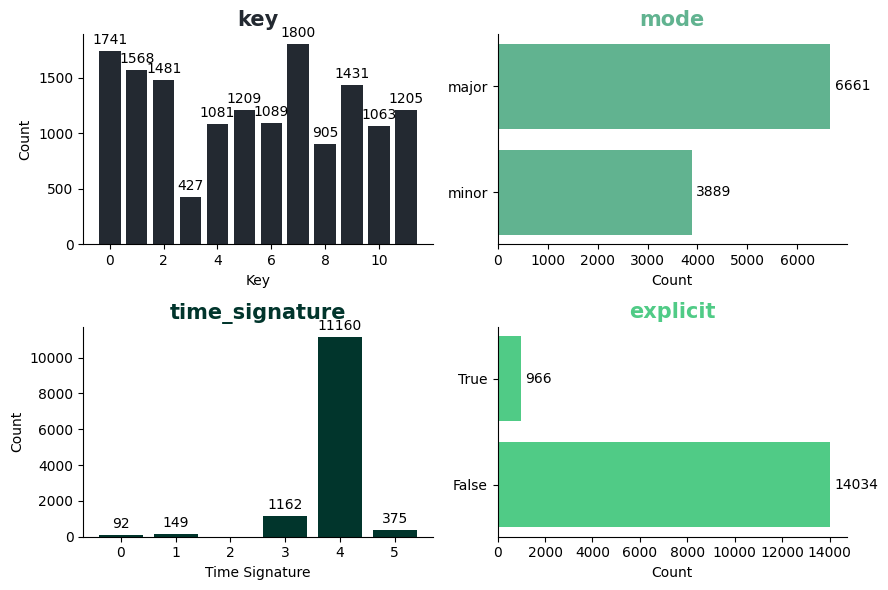
\includegraphics[scale=0.35]{img/categorical_bars.png}
        \caption{Distribution of discrete and binary variables.}
        \label{fig:enter-label}
    \end{minipage}
    \hfill
    \begin{minipage}{0.45\textwidth}
        \centering
        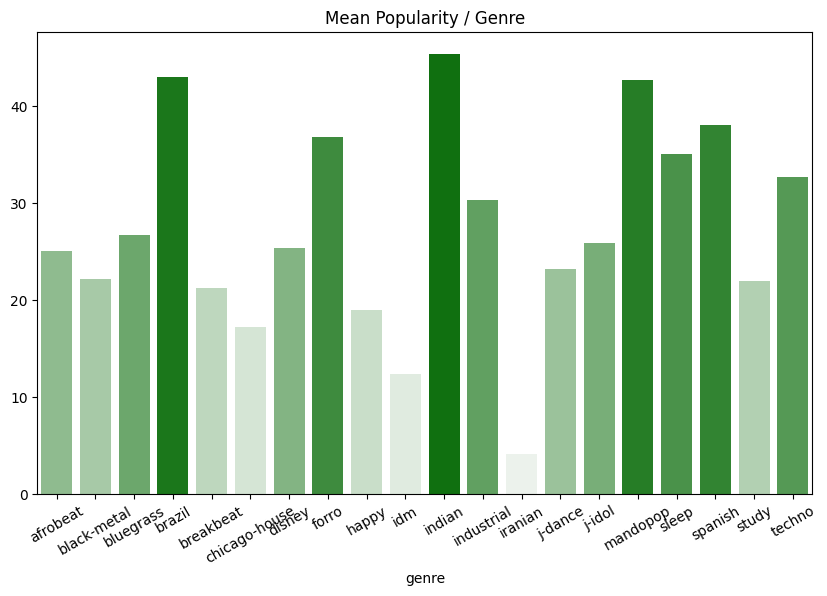
\includegraphics[scale=0.35]{img/popularity_genre.png}
        \caption{Mean popularity of tracks by genre.} 
        \label{fig:enter-label2}
    \end{minipage}
\end{figure}

Most of the tracks are in 4/4, and the keys C (0) and G (7) stand out, with a prevalence of major modes. Also noticeable is the sparse presence of songs with explicit content. By looking at the summary statistics of the continuous variables, we can calculate skewness and excess kurtosis. Excess kurtosis describes the shape of the tail of a distribution, while skewness measures the symmetry of the distribution. We can see that:
\begin{itemize}
\item \texttt{duration\_ms} has a high kurtosis ($161.5$) and positive skewness ($7.74$), indicating that most values are concentrated to the left of the mean with a long tail to the right;
\item \texttt{popularity}, \texttt{danceability}, \texttt{energy}, \texttt{acousticness}, \texttt{instrumentalness}, \texttt{val-\\*ence}, \texttt{tempo}, and \texttt{processing} have negative excess kurtosis, indicating that the distribution is flatter compared to a normal distribution;
\item \texttt{loudness}, \texttt{speechiness}, \texttt{liveness}, \texttt{n\_beats}, and \texttt{n\_bars} have positive excess kurtosis, indicating that the distribution has heavier tails and a sharper peak compared to a normal distribution;
\item There is no sufficient available data for \texttt{popularity\_confidence}.
\end{itemize}
\begin{comment}
\begin{figure}[!htb]
   \begin{minipage}{0.48\textwidth}
     \centering
     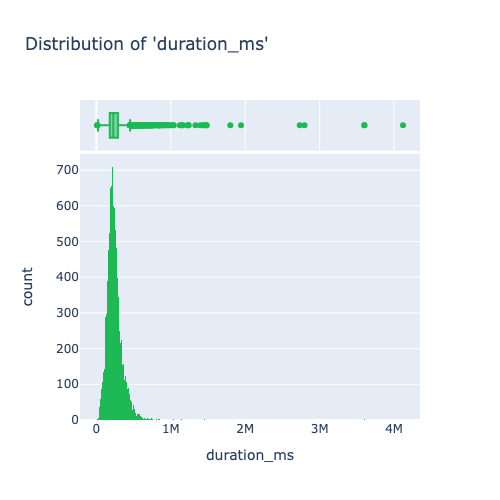
\includegraphics[width=\linewidth]{img/durationms_hist.png}
     \caption{Distribution of the feature 'duration\_ms'}\label{Fig:durationms_hist}
   \end{minipage}\hfill
   \begin{minipage}{0.48\textwidth}
     \centering
     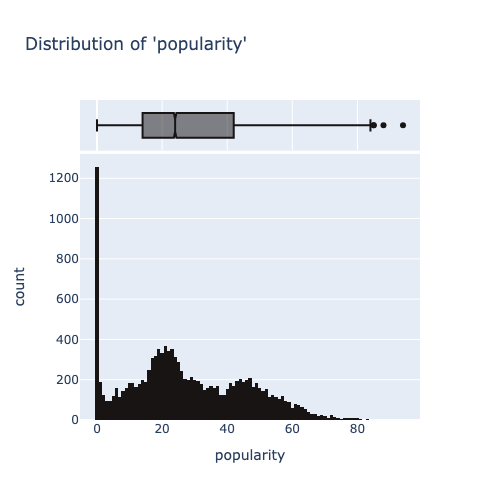
\includegraphics[width=\linewidth]{img/popularity_hist.png}
     \caption{Distribution of the feature 'popularity'}\label{Fig:popularity_hist}
   \end{minipage}
\end{figure}
\end{comment}

\section{Outliers detection}
\label{outliers_detection}
In order to check for possible outliers within the dataset, we can use some statistical tools, such as standard deviation and IQR (Interquartile Range), to measure the variability of data. The standard deviation method considers any data point that is a certain number of standard deviations away from the mean as an outlier; IQR is the range between the first and the third quartiles (namely $Q1$ and $Q3$): $\text{IQR} = Q3-Q1$. The data points which fall below $Q1-1.5*\text{IQR}$ or above $Q3+1.5*\text{IQR}$ may be candidate outliers.\\
We identified which features in the dataset have potential outliers according to both methods. We can view boxplots related to some of these features:
\begin{figure}[H]
    \centering
    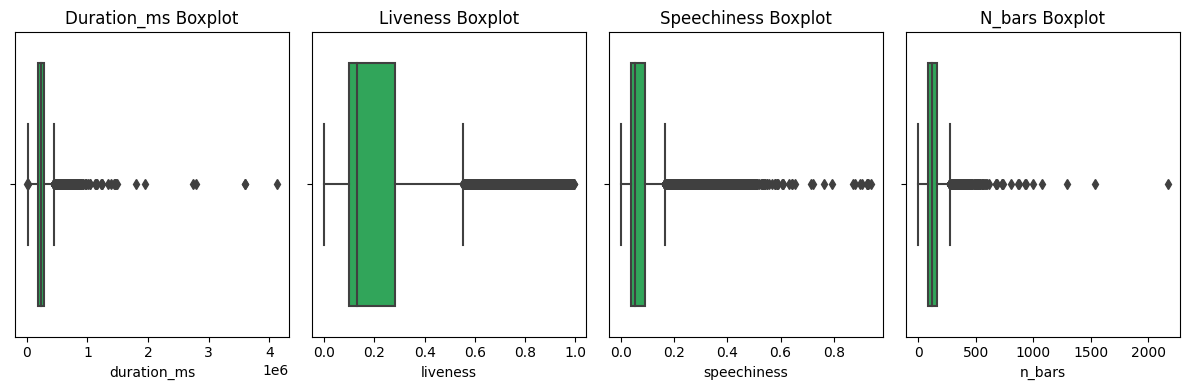
\includegraphics[scale=0.4]{img/boxplots.png}
    \caption{Some of the features with more presence of outliers according to the statistical methods used.}
    \label{fig:enter-label}
\end{figure}
The large presence of outliers for features such as \texttt{duration\_ms}, \texttt{liveness} and \texttt{speechiness} led us to check the details of the various candidate outliers: in fact, they actually refer to live recordings, DJ sets or compilations (like study background music). In this phase, we’ve decided not to remove any records, as doing so would result in a loss of approximately $44.59\%$ of the samples.
\newpage
\section{Handling missing values}
\begin{figure}[H]
    \centering
    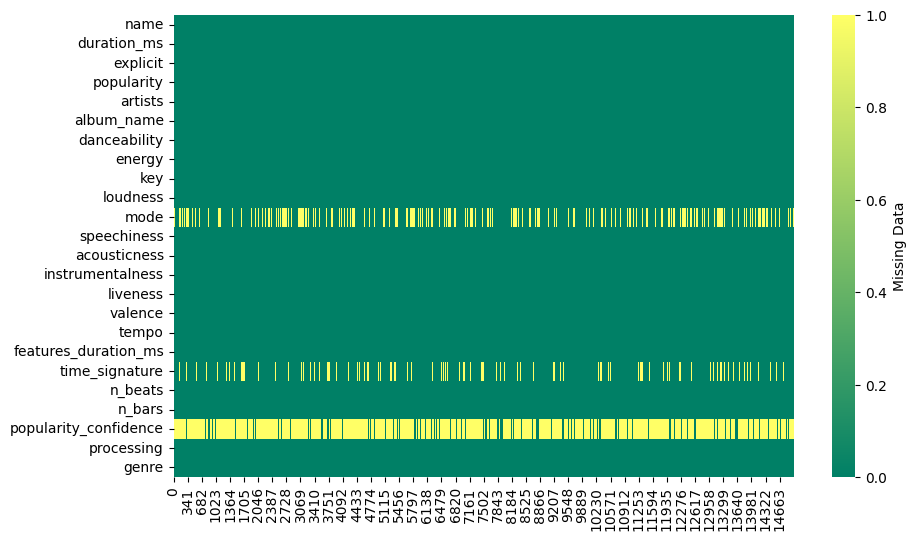
\includegraphics[scale=0.6]{img/missing_values.png}
    \caption{Heatmap of the data coded as boolean for "missing-ness" (1 is missing, 0 is not). Here we use the transposed boolean dataframe with \texttt{isna()} as input of the Seaborn’s \texttt{heatmap()} function.}
    \label{fig:missing-values}
\end{figure}
\begin{itemize}
\item \texttt{popularity\_confidence}: since 12783 values ($85.22\%$ of the total) turn out to be missing, we therefore decided to drop the column from the original dataset, because it may not contain any information about the data.
\item \texttt{mode}: the column contains binary values. Of these, $63.14\%$ are $1$ and $36.86\%$ are $0$. We decided to replace the null values by randomly inserting $0$ or $1$ while maintaining the percentage of the two classes. Although it might be formally wrong to assign 'minor' or 'major' even to track types such as live recordings or compilations, we noticed that among the nonmissing records it had already been done, so we simply chose to keep the percentage of classes. In this way we prevented the deletion of records that could be used in the next analysis and at the same time maintained the distribution of classes without altering the dataset.
\item \texttt{time\_signature}: we checked the Spotify Web API documentation in order to get more specific information about the variables. In the "Tracks" section, time\_signature is described as an estimated time signature ranging from 3 to 7, indicating time signatures from "3/4" to "7/4" . Time signature (or meter) is a notation convention for specifying the number of beats in each measure (or measure). So we may decide to reject the variable, as it can be calculated from two other variables in the dataset (n\_beats and n\_bars). In order to verify this choice, we tested the calculation on a copy of the dataset, filtered with only non null values. The accuracy is calculated as the percentage of recalculated values corrected (i.e., with the value equal to the true value of time\_signature). The result is: \mintinline{python}|Accuracy Rate: 95.90|\%. We can therefore consider the formula reliable and drop the column as the feature can be derived.
\end{itemize}

\section{Dependencies and correlations}
\begin{figure}[H]
    \centering
    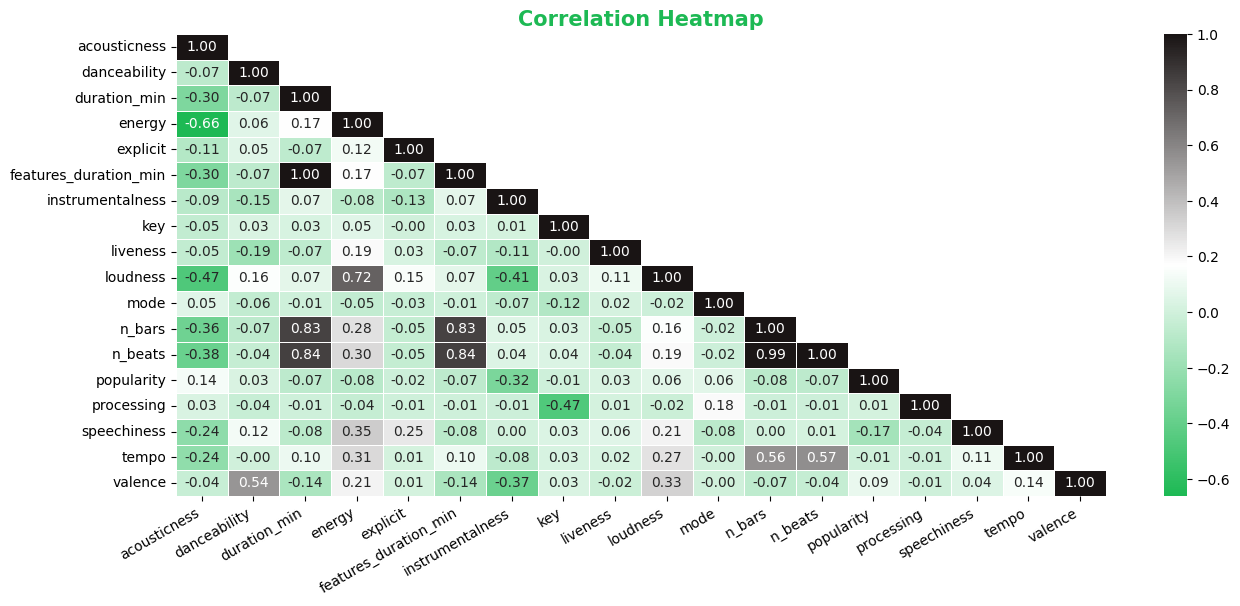
\includegraphics[scale=0.45]{img/corr_heatmap.png}
    \caption{Spearman's correlation heatmap of features.}
    \label{fig:enter-label}
\end{figure}
After dropping duration\_ms and features\_duration\_ms because durations in minutes were introduced, we can see that the correlation matrix confirms that longer songs typically have more beats and bars. Energetic songs tend to be louder, while acoustic songs have lower energy. Instrumental tracks generally have lower energy and loudness. Valence is positively related to danceability and tempo, suggesting happier songs are more danceable and faster-paced. Faster-tempo songs are also more danceable. We can also drop the "features\_duration\_min" column because it has virtually maximum positive correlation with "duration\_min".\\
\\
Once we had filtered the dataset by selecting and standardizing (using the StandardScaler from \texttt{sklearn.preprocessing}) only continuous variables, we decided to implement a PCA (from \texttt{sklearn.decomposition}) to look for additional relationships between variables and identify the linear combinations of original variables that explain most of the variance in the data. After visualizing the scree plot, considering the elbow rule, we can rerun the PCA with 3 components and interpret the results. The results of the PCA, and the loadings of the original variables on the first three principal components are organized into new dataframes. \\
This procedure leads to the following results:
\begin{figure}[H]
    \begin{minipage}{0.5\textwidth}
        \centering
        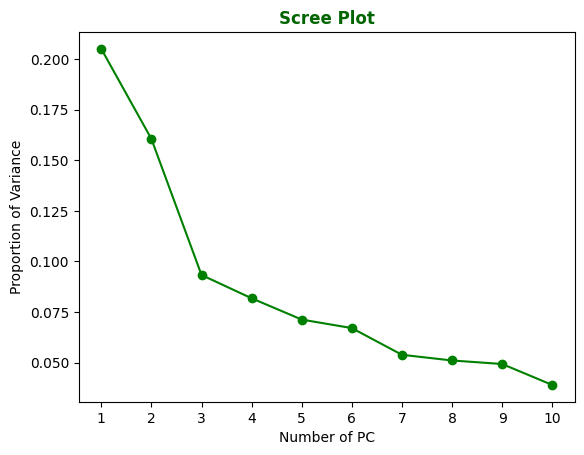
\includegraphics[scale=0.4]{img/scree_plot.png}
        \caption{The scree plot shows how much each principal component contributes to the total variance of the data.}
    \end{minipage}
    \hfill
    \begin{minipage}{0.5\textwidth}
        \begin{table}[H]
            \tiny
                \centering
            \begin{tabular}{|l|l|l|l|}
                \hline
                \textbf{Feature} & \textbf{PC1} & \textbf{PC2} & \textbf{PC3} \\
                \hline
acousticness & -0.36 & 0.14 & 0.03 \\
danceability & 0.15 & \textbf{-0.33} & 0.00 \\
duration\_min & 0.31 & \textbf{0.39} & 0.02 \\
energy & \textbf{0.39} & -0.23 & -0.02 \\
explicit & 0.06 & -0.14 & -0.04 \\
instrumentalness & -0.14 & 0.31 & -0.15 \\
key & 0.05 & -0.03 & \textbf{-0.62} \\
liveness & 0.03 & -0.03 & 0.04 \\
loudness & 0.36 & -0.33 & 0.04 \\
mode & -0.04 & 0.02 & 0.36 \\
n\_bars & \textbf{0.40} & \textbf{0.38} & 0.04 \\
n\_beats & \textbf{0.41} & 0.36 & 0.04 \\
popularity & -0.04 & -0.11 & 0.13 \\
processing & -0.03 & 0.02 & \textbf{0.65} \\
speechiness & 0.06 & -0.15 & -0.08 \\
tempo & 0.31 & -0.00& 0.05 \\
valence& 0.15& \textbf{-0.37}& 0.06\\
                \hline
            \end{tabular}
            \caption{Principal Component Loadings}
        \end{table}
    \end{minipage}
\end{figure}
\noindent PC1 is influenced by n\_beats, n\_bars, and energy, so it might be viewed as a measure of the rhythm intensity of the track. PC2 is positively influenced by duration\_min and n\_bars, and negatively influenced by valence and danceability: it might be seen as contrasting measure of song duration and rhythm structure with the mood and danceability of the music. PC3 is influenced by processing and negatively influenced by key, it might be viewed as a measure of the key’s impact on the processing of the music. This is an interpretation of the results with the understanding that PCA is a "black box": since we do not know the procedure behind the algorithm's choice of PCs, we are giving a hypothesis that can later be confirmed or discarded during. Before continuing, we can further select the variables in the dataset: as we dropped time\_signature, by the same reasoning we can drop n\_beats, because it can be derived from the product $\texttt{duration\_min}*\texttt{tempo}$ (which is in fact expressed in beats per minute, BPM). Entering the second phase of the analysis, we decided to normalize all variables using Z-Score normalization (\texttt{StandardScaler} class from the \texttt{sklearn.preprocessing} module), since is less sensitive than Min-Max to the presence of outliers. This is the description of the dataset at the end of the data understanding phase:\\
\begin{center}
\begin{tiny}
\begin{tabular}{|l|l|l|l|l|l|l|l|l|l|}
\hline
\textbf{index} & \textbf{count} & \textbf{mean} & \textbf{std} & \textbf{min} & \textbf{25\%} & \textbf{50\%} & \textbf{75\%} & \textbf{max} \\
\hline
name & 15000 & 7499.5 & 4330.271 & 0 & 3749.75 & 7499.5 & 11249.25 & 14999 \\
explicit & 15000 & 0.064 & 0.245 & 0 & 0 & 0 & 0 & 1 \\
popularity & 15000 & 0 & 1 & -1.475 & -0.722 & -0.184 & 0.784 & 3.582 \\
artists & 15000 & 1987.648 & 1755.411 & 0 & 486 & 1437 & 3178 & 6256 \\
album\_name & 15000 & 4084.496 & 2832.827 & 0 & 1569.75 & 3673 & 6399 & 9819 \\
danceability & 15000 & 0 & 1 & -2.837 & -0.567 & 0.149 & 0.741 & 2.208 \\
energy & 15000 & 0 & 1 & -2.482 & -0.667 & 0.2 & 0.862 & 1.3 \\
key & 15000 & 0 & 1 & -1.475 & -0.917 & -0.08 & 0.757 & 1.593 \\
loudness & 15000 & 0 & 1 & -6.766 & -0.29 & 0.265 & 0.632 & 2.007 \\
mode & 15000 & 0.628 & 0.483 & 0 & 0 & 1 & 1 & 1 \\
speechiness & 15000 & 0 & 1 & -0.966 & -0.536 & -0.378 & 0.056 & 9.863 \\
acousticness & 15000 & 0 & 1 & -0.922 & -0.893 & -0.452 & 0.817 & 2.1 \\
instrumentalness & 15000 & 0 & 1 & -0.749 & -0.749 & -0.741 & 1.194 & 1.863 \\
liveness & 15000 & 0 & 1 & -1.11 & -0.609 & -0.439 & 0.324 & 3.98 \\
valence & 15000 & 0 & 1 & -1.576 & -0.869 & -0.075 & 0.819 & 2.013 \\
tempo & 15000 & 0 & 1 & -3.856 & -0.726 & 0.034 & 0.591 & 3.051 \\
n\_bars & 15000 & 0 & 1 & -1.709 & -0.604 & -0.152 & 0.407 & 27.181 \\
processing & 15000 & 0 & 1 & -1.197 & -0.848 & -0.38 & 0.948 & 1.54 \\
genre & 15000 & 0 & 1 & -1.648 & -0.824 & 0 & 0.824 & 1.648 \\
duration\_min & 15000 & 0 & 1 & -1.861 & -0.522 & -0.148 & 0.329 & 30.264 \\
\hline
\end{tabular}
\end{tiny}
\end{center}



\stepcounter{chapter} % This line will increment the chapter counter
\chapter*{Clustering} % This line will create an unnumbered chapter
\addcontentsline{toc}{chapter}{\protect\numberline{\thechapter}Clustering} % This line will add the chapter to your table of contents
\markboth{Clustering}{} % This line will set the header
\vspace{-10mm}
Before starting the cluster analysis, we selected the variables in the dataset, dropping nominal ones, i.e., \texttt{name}, \text{album\_name}, \text{artists} and categorical/discrete ones (like \texttt{key} and \texttt{genre}). We decided to also drop the \texttt{processing} column because, observing the number of unique values and the distribution, is likely to be discrete (like key and time signature); moreover we don't have an accurate description of the variable, so it would be difficult to give an interpretation to its possible contribution in a cluster (although from the PCA there was a glimpse of a contribution in relation to key). The remaining features are 12: ['duration\_min', 'popularity', 'danceability', 'energy', 'loudness', 'speechiness', 'acousticness', 'instrumentalness', 'liveness', 'valence', 'tempo', 'n\_bars'].\\
The clustering techniques were applied to two datasets: one with 15000 records and 12 features, and another with 10575 records and 12 features, excluding outliers (rejected based on the criteria described in Data Understanding, IQR and Standard Deviation, see \ref{outliers_detection}); the cutoff this time is smaller (about 29\% of the samples) because we dropped some columns that contained the outliers that were cut in the first case. Henceforth we will call $\mathbf{F}$ the full dataset with all samples and $\mathbf{C}$ the cut dataset without outliers. The best performing dataset was chosen for each algorithm. The process involved three steps: using all features, using only selected features, and evaluating performance. The selected features were determined by a selection algorithm based on feature importance for cluster separation (see Fig. \ref{fig:parallel}).
\section{Centroid-based clustering}
\subsection{Choice of $k$}
We applied the following techniques for choosing the optimal value of $k$, both methods provide heuristic approaches to determine the number of clusters.
\begin{figure}[ht]
\begin{minipage}{.6\textwidth}
\textsc{Elbow Method}: involves running the k-means algorithm for a choosen range of values of $k$. For each value of $k$, the Sum of Squared Errors (SSE) is calculated and stored in a list. The SSE tends to decrease toward 0 as we increase $k$ (i.e., as the number of clusters increases, the distance from each data point to its closest centroid gets smaller). The “elbow” in the plot of SSE versus $k$ is considered as an indicator of the appropriate number of clusters. This “elbow” is the point representing the value of $k$ beyond which the decrease of SSE is no longer evident. When the elbow point is not distinguishable, we can use \texttt{KneeLocator} from the library \texttt{kneed}.
\end{minipage}
\begin{minipage}{.4\textwidth}
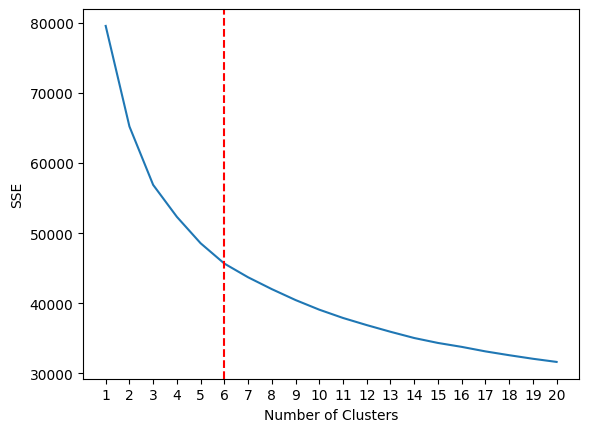
\includegraphics[width=\textwidth]{img/sse_all.png}
\end{minipage}
\end{figure}
\begin{figure}[ht]
\begin{minipage}{.6\textwidth}
\textsc{Silhouette Method}: measures (range -1 to 1) how similar an object is to its own cluster compared to other clusters; a high value indicates that the object is well matched to its own cluster and poorly matched to neighboring clusters. If most objects have a high value, then the clustering configuration is appropriate. In this analysis the silhouette is calculated using a precomputed euclidean distance matrix (we used \texttt{pdist}, \texttt{squareform} from \texttt{scipy.spatial.distance}).
\end{minipage}
\begin{minipage}{.4\textwidth}
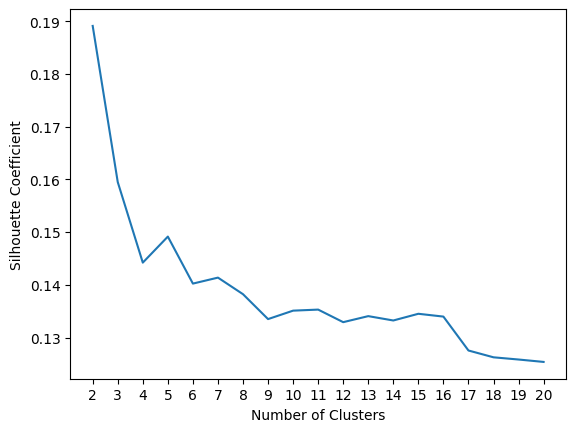
\includegraphics[width=\textwidth]{img/sil_all.png}
\end{minipage}
\end{figure}
\newpage
\subsection{Evaluation techniques}
Clustering evaluation is first performed by calculating \textbf{SSE} and \textbf{silhouette score}, for both datasets. For further validation we implemented a code that provides a thorough evaluation of the KMeans clustering results, taking into account the possibility of obtaining similar results by chance:
\begin{enumerate}
\item \textbf{Compute Correlation:} correlation (using the Pearson correlation coefficient) between the distance matrix of the data and the ideal similarity matrix, that is a binary matrix where 1 indicates that two points belong to the same cluster and 0 otherwise. 
\item \textbf{KMeans Evaluation:} we then evaluate the significance of the clustering result by comparing it with the results of clustering on randomized datasets. This is done by: randomizing the data, computing the KMeans clustering for the randomized data, computing SSE and correlation for the randomized data, storing the results and repeating the steps for a choosen number of permutations ($200$ for SSE evaluation, $100$ for Silhouette).
\item \textbf{Plots:} histogram and Kernel Density Estimation (KDE) plot of SSE and correlations for the randomized datasets. The original values of SSE and correlation are represented by a dashed vertical line. 
\end{enumerate}
If the original SSE is significantly lower than the permuted ones, it suggests that the clusters found by K-means are meaningful and not a result of random chance. On the other hand, if the original SSE is not much lower than the permuted ones, it suggests that the K-means solution might not be capturing any meaningful structure in the data. Then, if the original correlation is significantly different from the mean value given by permutations, it suggests that the clusters found by K-means are meaningful and not a result of random chance.

\subsection{K-Means}
Based on the assumptions above, for all the $12$ features the results are: $k=4$ for $\mathbf{F}$-dataset and $k=5$ for $\mathbf{C}$-dataset. The one that performed slightly better (but still poor, sil$=0.21$) is $\mathbf{F}$, with the following parallel chart:
\begin{figure}[H]
    \centering
    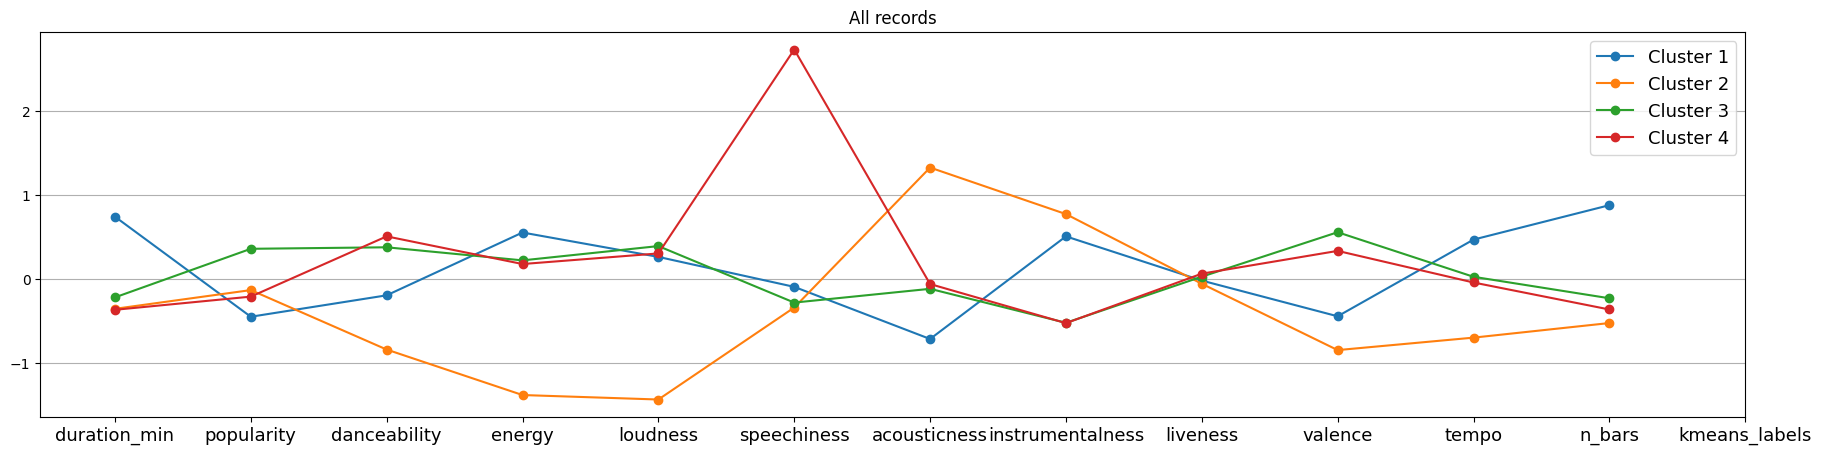
\includegraphics[scale=0.35]{img/parallel_all_kmeans.png}
    \caption{Parallel Line Chart; full dataset with all features. Points represents centroids with respect to the features.}
    \label{fig:parallel}
\end{figure}
\begin{wrapfigure}{r}{0.35\textwidth}
\vspace{-1cm}
\caption{2D and 3D plots: full dataset with selected features.}
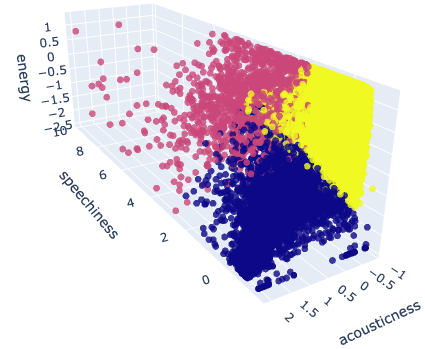
\includegraphics[width=\linewidth]{img/3d_kmeans.png}
\vspace{2cm}
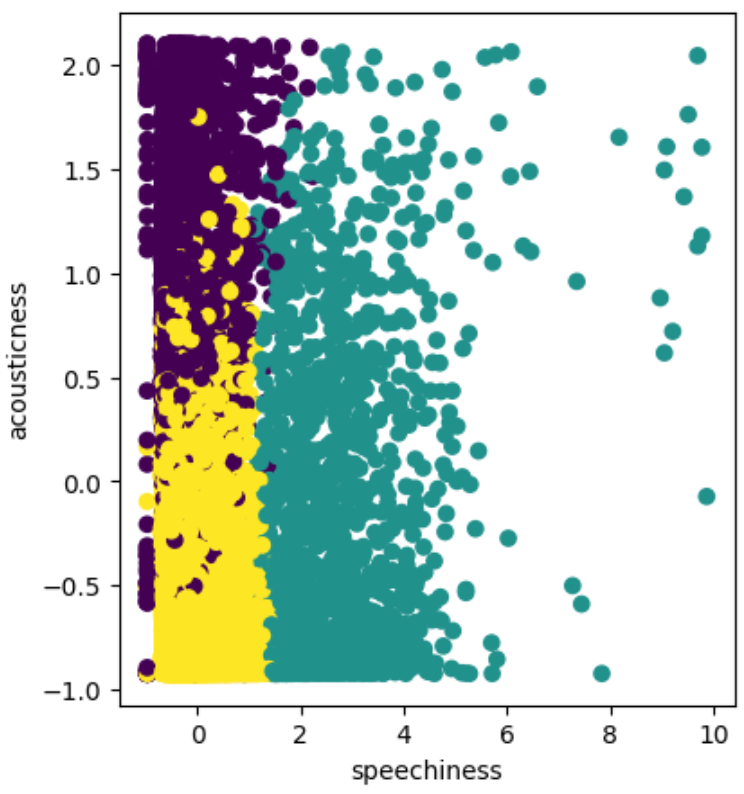
\includegraphics[width=0.7\linewidth]{img/2d_kmeans.png}
\vspace{-5cm}
\end{wrapfigure}
We decided to try to select only those features that generate more pronounced separation between centroids (either based on the parallel chart display or by calculating them with an appropriate algorithm). For the two datasets they were found to be more "important":
\begin{verbatim}
F -> ['speechiness', 'acousticness', 'energy']
C -> ['instrumentalness', 'acousticness', 'energy']
\end{verbatim}
Combinations with the 6, 5, or 4 most important features have been tested, but the results are poor. So we repeat the analysis using only the 3 most important features for each dataset. From the study of the SSE and silhouette score we obtain $k_\mathbf{F}=3$ and $k_\mathbf{C}=4$. \\
After fitting the two kmeans, the best silhouette score is $0.51$ ($\mathbf{F}$-dataset). As specified above, for further validation, correlations and SSE are calculated through permutations of the same data.
\begin{figure}[H]
\vspace{0.5cm}
    \centering
    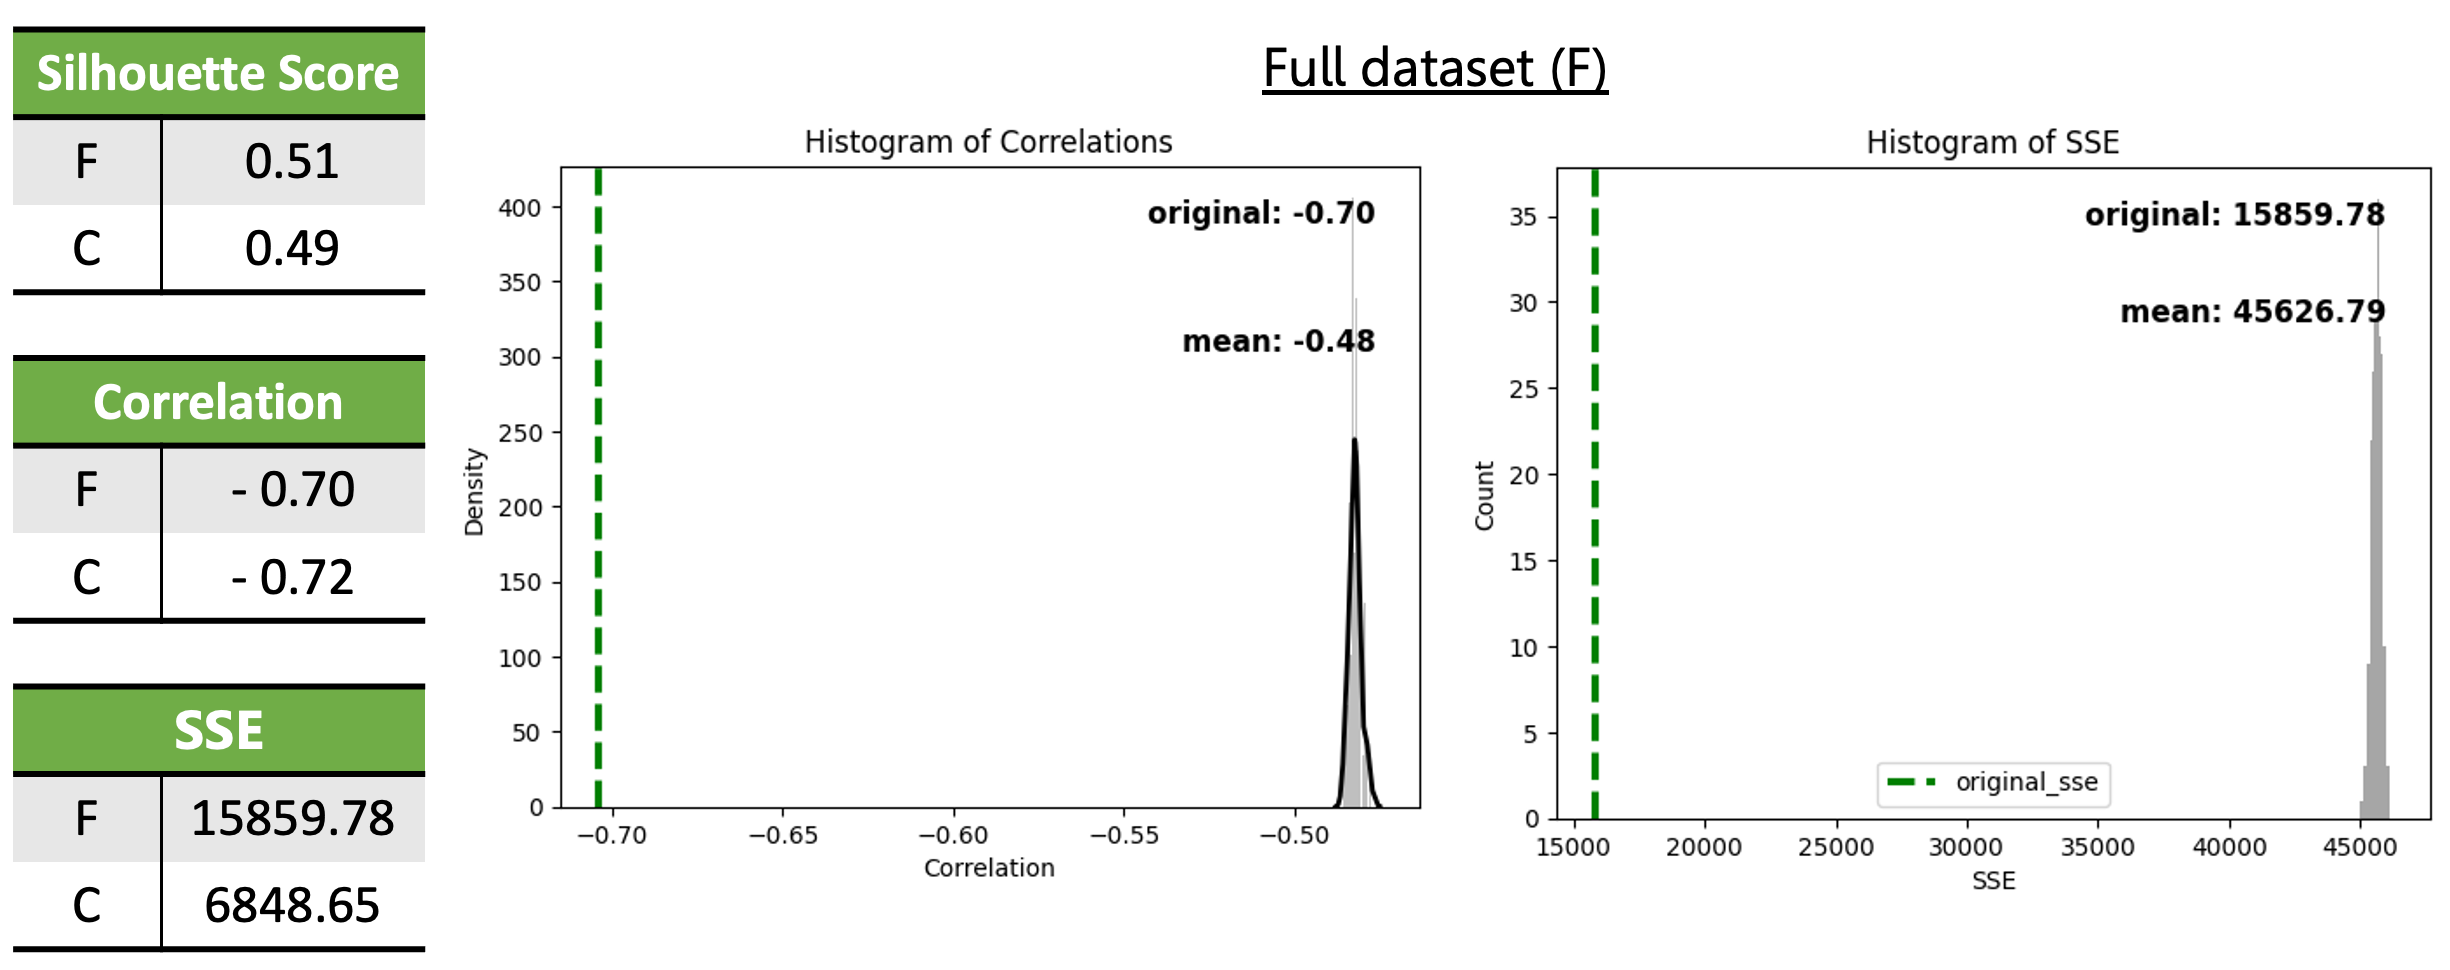
\includegraphics[scale=0.35]{img/final_kmeans.png}
    \caption{Results of KMeans evaluation, the histogram plot refers to the full dataset. F: full dataset, C: dataset without outliers.}
    \label{fig:enter-label}
\end{figure}
Both datasets show a negative correlation because it's calculated between the distance matrix and the ideal similarity matrix. We can try to give an interpretation to the clusters generated by the analysis:\\
\begin{wrapfigure}{l}{0.4\textwidth}
\vspace{-0.8cm}
    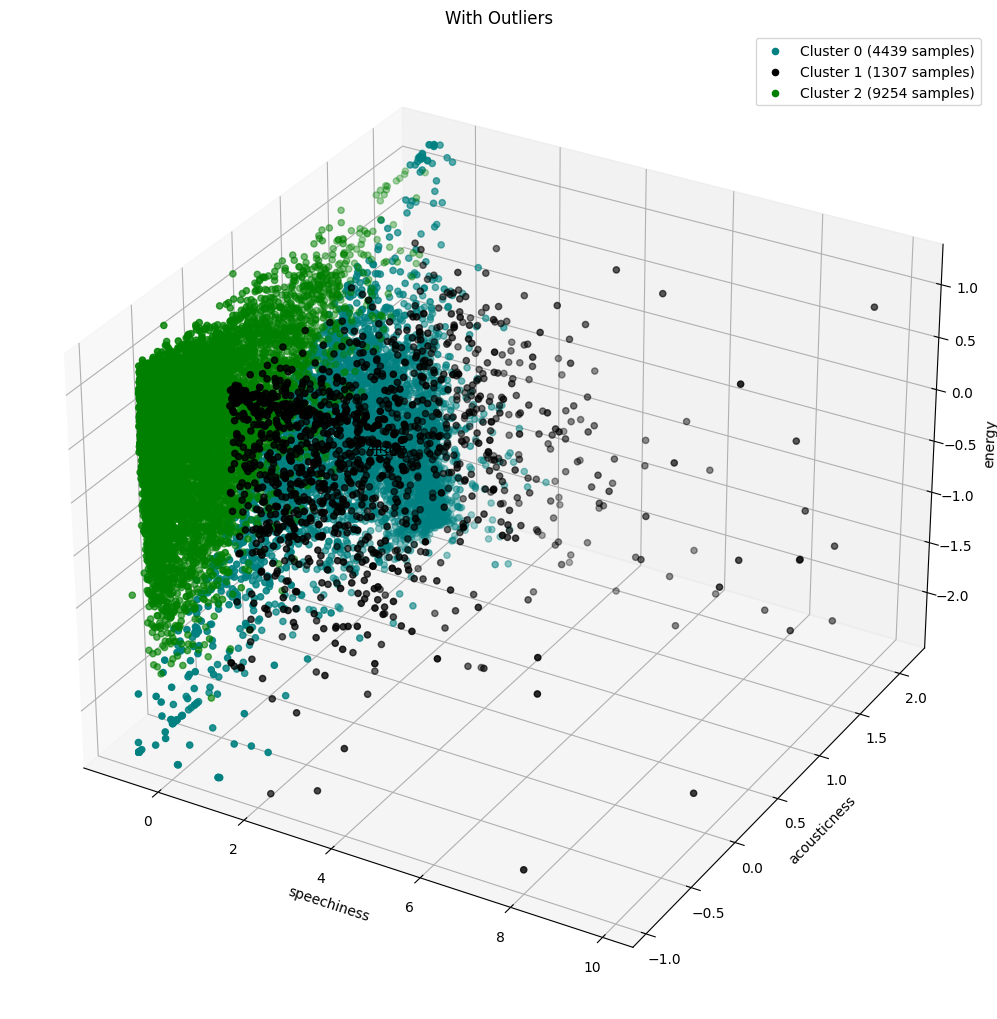
\includegraphics[width=\linewidth]{img/kmeans_FINALE.png}
\caption{Teal: Cluster 0, Black: Cluster 1, Green: Cluster 2}
\vspace{-2cm}
\end{wrapfigure}
\begin{itemize}
    \item Cluster \texttt{0}: \textbf{4439} samples; tracks with low energy and speechiness and high acousticness, it could contain mainly instrumental low-energy acoustic songs.
    \item Cluster \texttt{1}: \textbf{1307} samples; tracks with ascending speechiness, high energy and low acousticness, maybe containing rap songs.
    \item Cluster \texttt{2}: \textbf{9254} samples; tracks with low speechiness and acousticness and high energy, it may contain dance music.
\end{itemize}
\subsection{Bisecting K-Means}
Bisecting k-means is a hybrid approach between Hierarchical Clustering and K-means Clustering. Instead of partitioning the data set into $k$ clusters in each iteration, bisecting k-means algorithm splits one cluster into two sub clusters at each bisecting step (by using k-means) until $k$ clusters are obtained.\\
\begin{wrapfigure}{l}{0.6\textwidth}
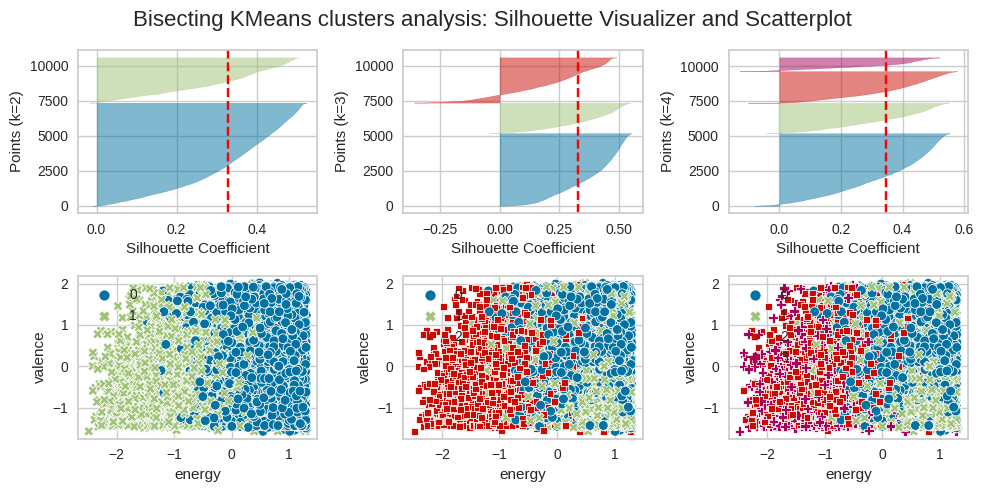
\includegraphics[width=\linewidth]{img/bkmeans_ev2.png}
\caption{Silhouette Visualizer, from $k=2$ to $k=4$.}
\label{bk_viz}
\end{wrapfigure}
In this section we performed the analysis with $k_\mathbf{F}=3$ and $k_\mathbf{C}=4$ and a varying number of features, from 12 down to 3 (based on importance), computing SSE and Silhouette Coefficient for each set of features. From the results, it appears that the $\mathbf{C}$ dataset (without outliers) performs better (but still gives bad performances) in terms of both SSE ($53130.08$) and Silhouette ($0.26$) for $4$ features: ['acousticness', 'energy', 'loudness', 'valence'] for $\mathbf{F}$ and ['instrumentalness', 'acousticness', 'energy', 'valence'] for $\mathbf{C}$. Although the results are bad (SSE greater than 50000), to attempt further visualization we used Silhouette Visualizer from the yellowbrick library, which generates a series of silhouette plots and scatterplots for a variable number of clusters (in this case 2 to 4, Fig. \ref{bk_viz}).
\section{Density-based clustering}
Density-based clustering algorithms like DBSCAN can identify clusters of arbitrary shapes in datasets. This is an advantage over other clustering algorithms that assume clusters are spherical or have other predefined shapes. Additionally, DBSCAN can handle noise and outliers in the data, and does not require the number of clusters to be specified in advance.
\subsection{DBSCAN}
Again we run the algorithms on both the full dataset ($\mathbf{F}$) and the dataset without outliers ($\mathbf{C}$) to compare performance, both scaled with StandardScaler. Both datasets are tested with all features and then with the previously chosen features for kmeans analysis. The other feature selections did not affect the final results much, so we assumed that using the same attributes might have led to a better comparison between the two algorithms.\\
In order to choose the best parameters, we determined the optimal value of epsilon (eps), by plotting the $k$-th nearest neighbor distances for each data point in a given dataset, and then using the “elbow method” to find the optimal eps value (using again \texttt{KneeLocator} from \texttt{kneed}).
\begin{figure}[H]
    \centering
    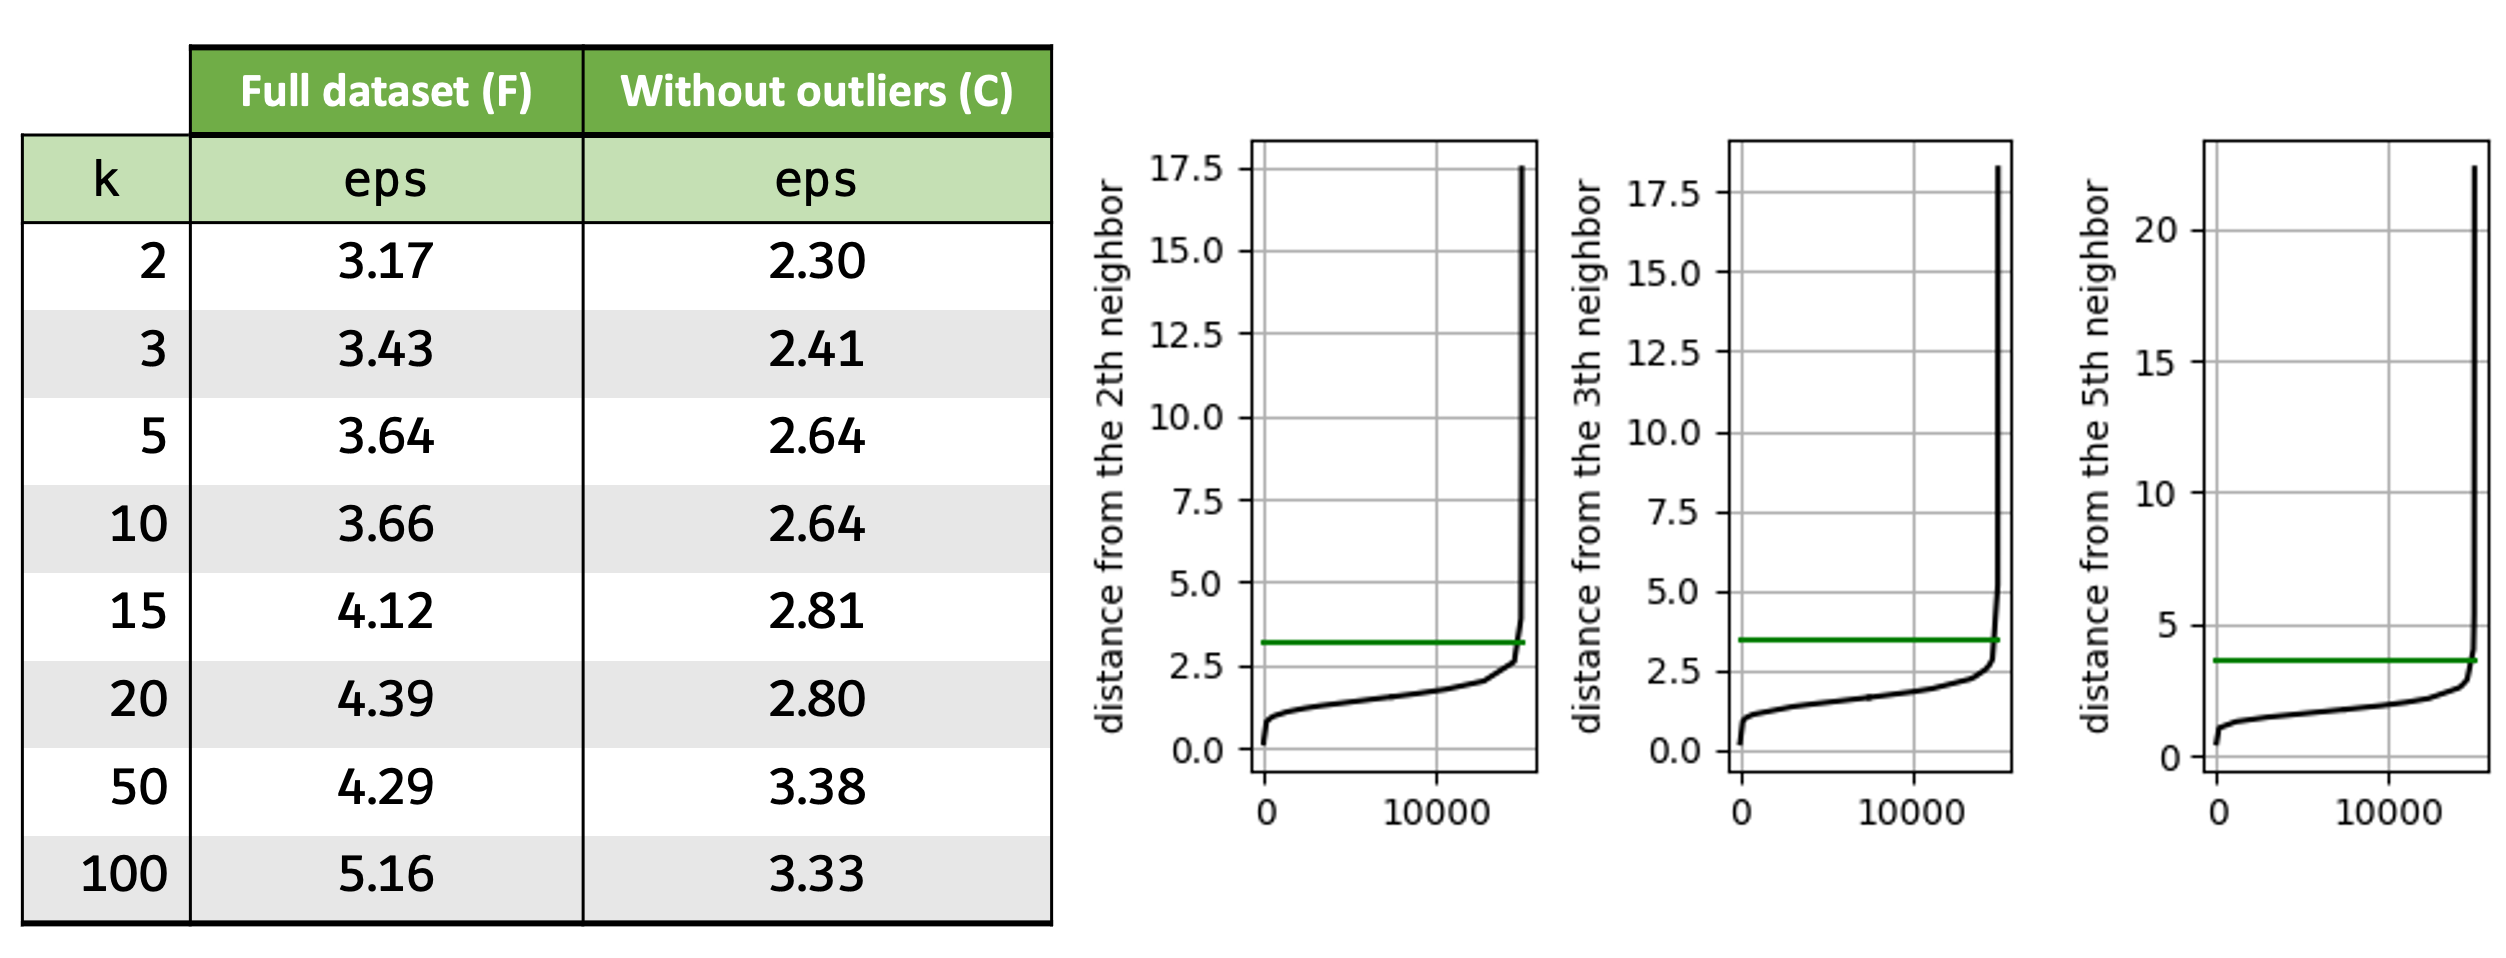
\includegraphics[scale=0.3]{img/eps_dbscan.png}
    \caption{Values of $k$ and \texttt{eps} for the datasets with all features.}
    \label{fig:enter-label}
\end{figure}
\begin{wrapfigure}{l}{0.4\textwidth}
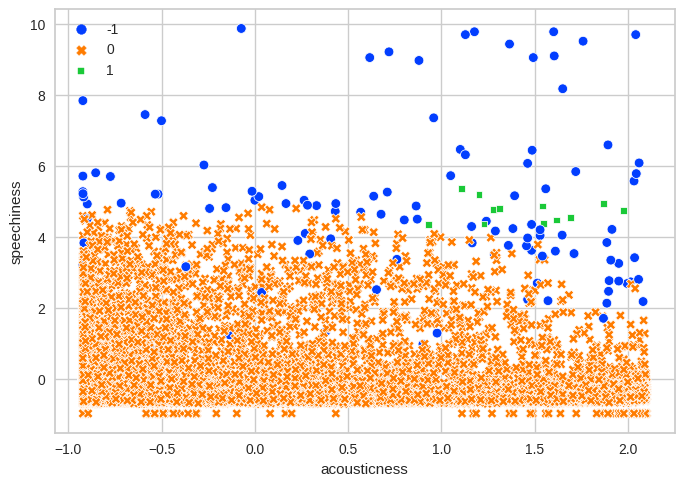
\includegraphics[width=\linewidth]{img/dbscan.png}
\caption{DBSCAN: Full Dataset, eps=0.75, minPts=12, sil\_score=0.59}
\vspace{-1cm}
\label{fig:dbscan}
\end{wrapfigure}
Because of the poor results with these configurations, we tried choosing a single eps value (average value of the two lists of values seen before, so $3.72$ for $\mathbf{F}$ and $2.10$ for $\mathbf{C}$) testing a wider range of k ($2$ to $51$) to find the winning combination. The best results are: \texttt{Full Dataset, eps=3.72, minPts=2, silhouette=0.45}.\\
Then we tried the same procedure by selecting, for each dataset, the same features selected for the kMeans (so we could make a better comparison); the results are: \texttt{Full Dataset, eps=0.75, minPts=12, silhouette=0.59}.\\
Despite having a convincing silhouette value, we discovered that the clustering is really very unbalanced (Fig. \ref{fig:dbscan}), since almost all the points are in the first cluster (orange), very few points are in the second cluster (green) and the others are all noise points (blue).
\section{Hierarchical clustering}
We decided to perform hierarchical clustering with Euclidean and Manhattan distances (precomputed) as metrics, and \texttt{single}, \texttt{complete}, \texttt{ward} and \texttt{average} linkages. By setting \texttt{n\_clusters}$=3$ (in order to compare results with KMeans analyisis), we used an algorithm that tested different combinations of distance-linkage returning a silhouette score. Also for the hierarchical clustering analysis, we tested the procedure first on the datasets with all features and then selecting the same features used for the second part of the KMeans. The best results were given by the configuration: dataset $\mathbf{F}$, \texttt{euclidean} distance, \texttt{single} linkage, $\texttt{sil\_score}=0.93$. The high value of silhouette score is unfortunately due to the large imbalance of the clusters: in fact, it is noticeable that there is a cluster that contains almost all the points in the dataset and then smaller clusters formed by single points. So we tried to see if the other linkages, although with lower silhouettes, could generate better separation.
\begin{figure}[H]
    \centering
    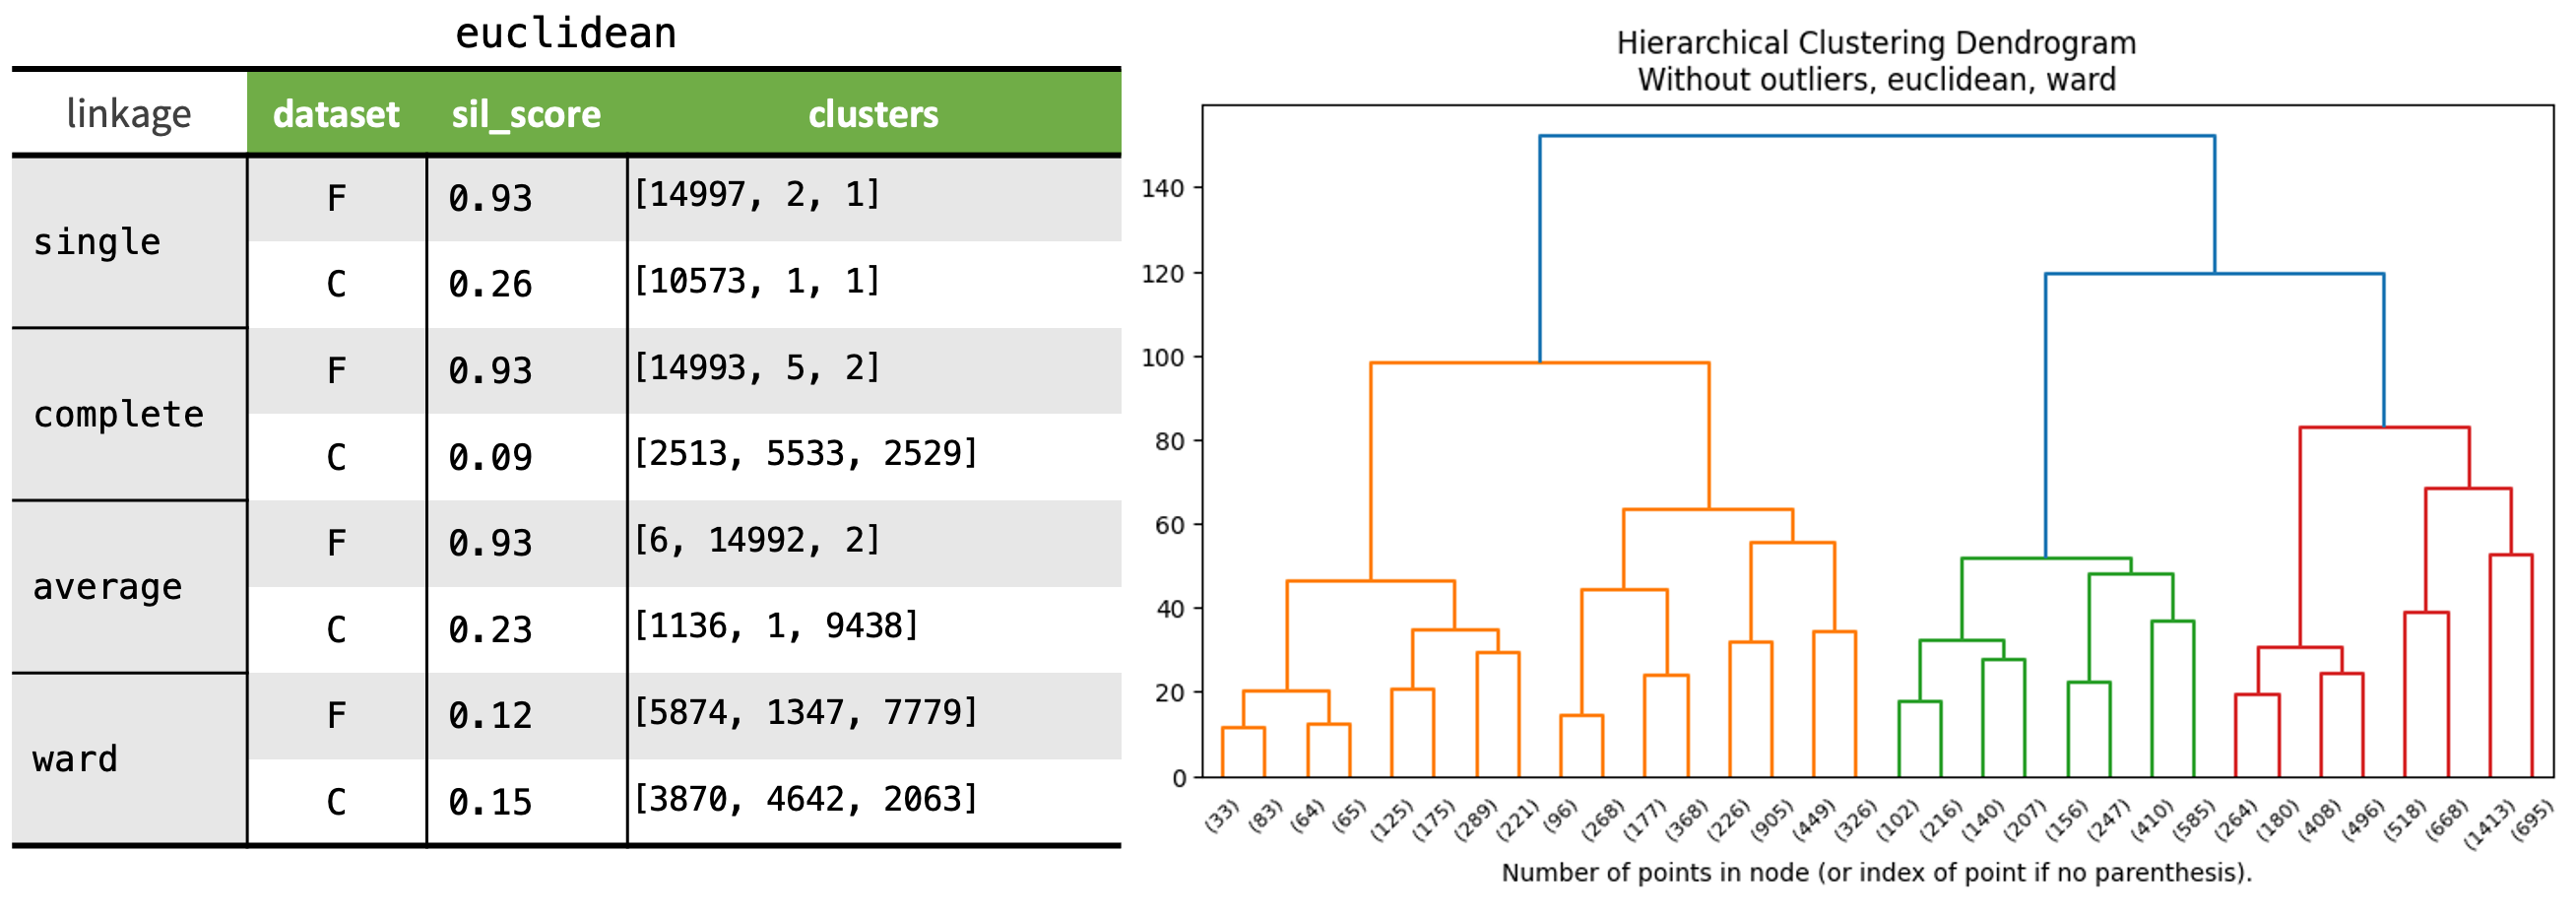
\includegraphics[scale=0.35]{img/hier_final2.png}
    \caption{Silhouette Scores of different combinations of dataset/linkage using euclidean distance.}
    \label{fig:enter-label}
\end{figure}
\noindent The C-euclidean-ward combination creates more balanced datasets, at the expense of a very low silhouette value.
\section{Final discussion}
Having reached this point, we can conclude that: DBSCAN is unable to provide optimal clustering, despite having tested several choices of eps and minPts, because it results mainly in large clusters that include almost the entire dataset, then only noise points; even the hierarchical methods produce highly unbalanced clusters. \\
\textbf{K-Means}, applied to a dataset with \textbf{selected features}, proved to be the only algorithm capable of separating some clusters in a balanced way with an acceptable silhouette value.
\stepcounter{chapter} % This line will increment the chapter counter
\chapter*{Classification} % This line will create an unnumbered chapter
\addcontentsline{toc}{chapter}{\protect\numberline{\thechapter}Classification} % This line will add the chapter to your table of contents
\markboth{Classification}{} % This line will set the header
\vspace{-10mm}
This section contains the methods applied to two different classification problems: the first target chosen is the variable \texttt{genre}, which contains 20 different classes; next we tried to apply the same algorithms to \texttt{popularity}, a continuous variable discretized into three classes (low, medium, high). For this analysis, the data were standardized using \texttt{StandardScaler} (from \texttt{sklearn.preprocessing}), and in a first step we chose to use all features in the dataset before making a selection: \textit{explicit}, \textit{popularity}, \textit{danceability}, \textit{energy}, \textit{key} (one-hot encoded), \textit{loudness}, \textit{mode}, \textit{speechiness}, \textit{acousticness}, \textit{instrumentalness}, \textit{liveness}, \textit{valence}, \textit{tempo}, \textit{n\_bars}, \textit{processing}, \textit{genre}, \textit{duration\_min}. Which could be an expected accuracy value for the classification of \texttt{genre}? A starting point might be a comparison with a random model: a model that randomly assigns classes would have an expected accuracy of $5\%$ (1 in 20); therefore, any model with significantly higher accuracy than this could be considered an improvement, even if it did not achieve an accuracy close to 1. The same is true for classification with three classes, where any model with accuracy greater than 1/3 can be considered acceptable (for purely analytical purposes) although perhaps not realistically usable.\\
For each classification algorithm presented, the work process was carried out in several successive stages: initially we apply a basic model with default parameters by measuring its accuracy, so as to have a starting value to be improved with appropriate choice of parameters; in fact, the second stage concerns the tuning of the hyperparameters using \texttt{GridSearchCV} by \texttt{sklearn.model\_selection}; once the model with the optimal parameters is obtained, we proceed with the evaluation. All the analysis presented were performed on the entire dataset used for the previous steps, appropriately split into \texttt{train} and \texttt{test} subsets. For some further tests, an external test dataset (never seen by the models), provided by the lecturer, was also used in order to have the three sets train, validation and test.
\subsubsection*{Evaluation metrics and techniques}
\begin{itemize}
    \item \textsc{Accuracy and Overall Error Estimate}: fraction of predictions got right by our model and relative error (1-accuracy).
    \item \textsc{Precision-recall curves}: trade-off between the rate of true positives and the positive predictive value for a predictive model using different probability thresholds.
    \item \textsc{F1 score}: measures the performance of a model that combines precision and recall. It ranges from 0 to 1, where 1 indicates perfect precision and recall. 
    \item \textsc{ROC-AUC score}: performance of a classification model at all classification thresholds. The area under the curve (AUC) measures the 2D area under the ROC curve, providing an aggregate measure of performance across all classification thresholds.
\end{itemize}
All the results provided refer to the performance measure on the test set.
\newpage
\section{Target: \texttt{genre}}
\vspace{-0.5cm}
\subsection{KNN}
\begin{wrapfigure}{r}{0.4\textwidth}
\centering
\vspace{-2cm}
\caption{ROC-AUC and Precision/Recall for KNN model.}
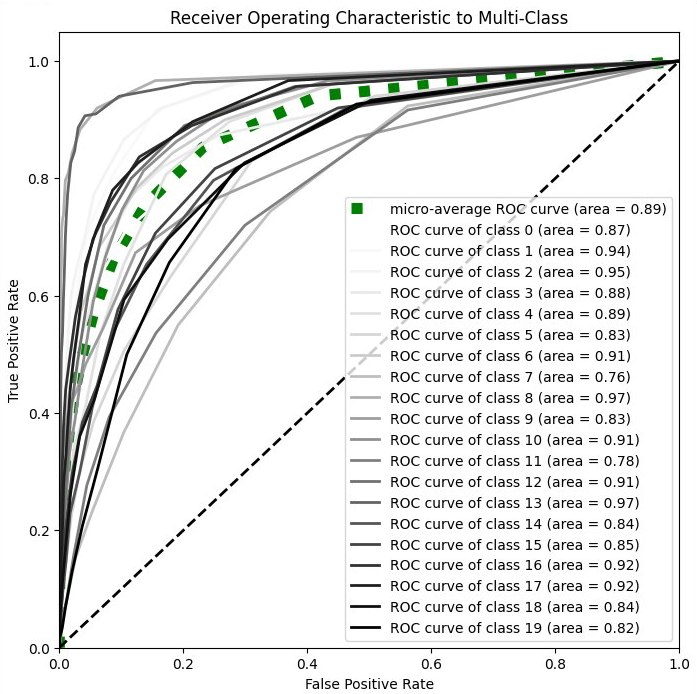
\includegraphics[width=0.8\linewidth]{img/roc_knn.jpg}
\vspace{2cm}
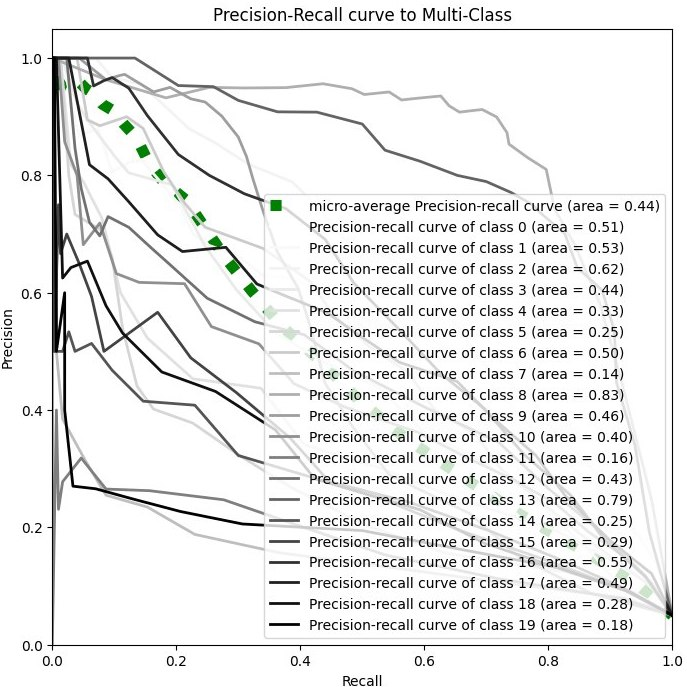
\includegraphics[width=0.8\linewidth]{img/pr_knn.jpg}
\vspace{-3cm}
\end{wrapfigure}

The base model returns an accuracy of $0.37$. For hyperparameter tuning, we start by looking at the trend of accuracy as the number of neighbors changes (from 1 to 100): the algorithm generates an error bar graph showing the average scores and their standard deviations for each number of neighbors and highlights the number of neighbors that obtained the highest accuracy, based on its cross-validation performance.
The configuration \texttt{\{'metric': 'cityblock', 'n\_neighbors': 26, 'weights': 'distance'\}} performs best according to GridSearch, with a final accuracy of about $0.48$.\\
\\
The model does not behave in the same way on the various classes, in particular it is better able to recognize tracks in the genre of "black metal" (class 2), "sleep" (class 8) and "study" (class 13).
\vspace{-0.5cm}
\subsection{Naive Bayes}
The Naive Bayes classifier is a classification algorithm based on Bayes' Theorem with the assumption that features are conditionally independent given the class label. In this study we distinctly use two types of NB: first, \texttt{Gaussian Naive Bayes}, a variant applicable to continuous variables in which attributes are assumed to follow a Gaussian distribution; it predicts the output variable based on each parameter independently. We then use \texttt{Categorical Naive Bayes}, suitable for discrete features that are categorically distributed.  
\begin{table}[H]
\centering
\footnotesize
\begin{tabular}{@{}|l|c|c|c|c|@{}}
\toprule
\rowcolor[HTML]{036400} 
{\color[HTML]{FFFFFF} \textbf{Classifier}} & \multicolumn{1}{l|}{\cellcolor[HTML]{036400}{\color[HTML]{FFFFFF} \textbf{Accuracy}}} & \multicolumn{1}{l|}{\cellcolor[HTML]{036400}{\color[HTML]{FFFFFF} \textbf{Precision}}} & \multicolumn{1}{l|}{\cellcolor[HTML]{036400}{\color[HTML]{FFFFFF} \textbf{Recall}}} & \multicolumn{1}{l|}{\cellcolor[HTML]{036400}{\color[HTML]{FFFFFF} \textbf{F1}}} \\ \midrule
\cellcolor[HTML]{C0C0C0}GaussianNB         & 0.37 & 0.37               & 0.37& 0.33                  \\ \midrule
\cellcolor[HTML]{C0C0C0}CategoricalNB & 0.40 & 0.38                           & 0.40 & 0.37                  \\ \bottomrule
\end{tabular}
\end{table}
\subsection{Decision Tree}
The base model returns a train accuracy of $1.0$ and a 
test accuracy $0.426$, with an obvious presence of overfitting. Before applying GridSearch we choose the ranges of some parameters based on the behavior of the model by plotting accuracy against different values: in particular we tuned \texttt{max\_depth}, \texttt{min\_samples\_split} and \texttt{min\_samples\_leaf}. The configuration with the optimal parameters turns out to be \texttt{\{'splitter': 'best', 'min\_samples\_split': 56, 'min\_samples\_leaf': 10, 'max\_depth': 11, 'criterion': 'gini'\}}, with an average accuracy of $0.45$. To visualize the tree we used \texttt{tree.export\_graphviz} from \texttt{sklearn} (below the graph is cut down to $\texttt{max\_depth}=2$ to make its content more understandable).
\begin{figure}[H]
    \centering
    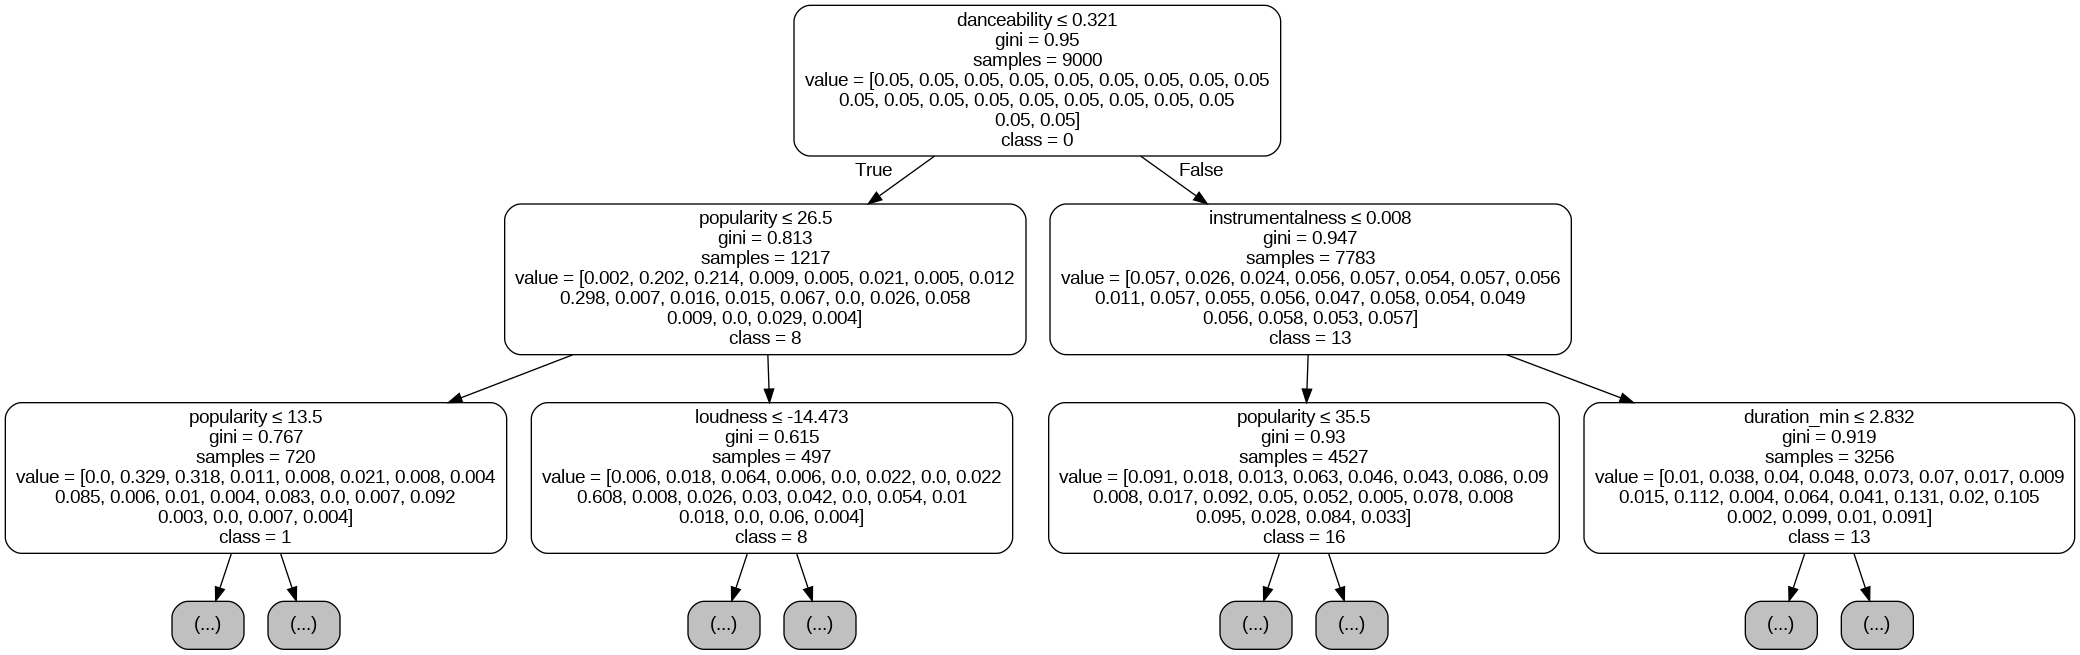
\includegraphics[scale=0.2]{img/decision_tree_genre_graphviz.png}
    \caption{Decision Tree with \texttt{genre} as target variable.}
    \label{fig:enter-label}
\end{figure}
\noindent We can also see the importance of features according to the model used: the most important is \texttt{popularity} ($0.23$), followed by \texttt{acousticness} ($0.13$), \texttt{danceability} ($0.13$), \texttt{duration\_min} ($0.12$) and so on; along with some features that have a very low contribution (like \texttt{liveness} or \texttt{processing}), we see that \texttt{key}, \texttt{explicit} and \texttt{mode} result useless (according to this model) in determining the genre of the track. We can therefore assume that the model relies mainly on how popular, acoustic and danceable a track is to identify its genre. Although predicting genre using popularity might be counterintuitive, removing it from features drops performance dramatically.\\ In a Decision Tree, when the parameter \texttt{ccp\_alpha} increases, more of the tree is pruned, thus creating a decision tree that generalizes better. So we implemented a procedure that could find the optimal value of the parameter. The result is [\texttt{Best ccp\_alpha value is:  0.000386}], but the performance of the model has not improved noticeably (accuracy about $0.46$).\\
We anticipated above that for an initial classification study we used all the features in the dataset. After seeing how all the models behaved, we decided to make a selection of the variables to be used: we used the correlation coefficient (the highest the correlation with target the highest the importance) and \texttt{mutual\_info\_classif} from \texttt{sklearn.feature\_selection}, that measures the reduction in entropy about one variable given the knowledge of another; in other words, it measures the dependency between each feature and the target variable. We used these two tools to obtain a combined score of each variable, so that we could select those with the highest score. From the results comes confirmation of the features identified by the decision tree; in fact, by selecting the 5 features with the highest score, we can repeat the analysis using only the variables \texttt{danceability}, \texttt{popularity}, \texttt{acousticness}, \texttt{energy}, \texttt{valence}. To recapitulate, the overall results are:
\begin{table}[H]
\centering
\footnotesize
\begin{tabular}{|l|c|c|c|c|c|}
\hline
\rowcolor[HTML]{036400} 
{\color[HTML]{FFFFFF} Decision Tree}      & {\color[HTML]{FFFFFF} Train acc} & {\color[HTML]{FFFFFF} Test acc} & {\color[HTML]{FFFFFF} precision} & {\color[HTML]{FFFFFF} recall} & {\color[HTML]{FFFFFF} F1} \\ \hline
\cellcolor[HTML]{C0C0C0}base model        & 1.0                              & 0.43                            & 0.43                             & 0.43                          & 0.43                      \\ \hline
\cellcolor[HTML]{C0C0C0}GridSearch        & 0.55                             & 0.45                            & 0.47                             & 0.46                          & 0.46                      \\ \hline
\cellcolor[HTML]{C0C0C0}ccp\_alpha        & 0.55                             & 0.46                            & 0.47                             & 0.46                          & 0.46                      \\ \hline
\cellcolor[HTML]{C0C0C0}Feature selection & 0.54                             & 0.46                            & 0.47                             & 0.46                          & 0.46                      \\ \hline
\end{tabular}
\end{table}
\subsection{Results}
\begin{itemize}
    \item KNN: [\texttt{accuracy}: $0.48$, \texttt{roc auc}: $0.89$, \texttt{precision/recall auc}: $0.44$]. Although we have improved the basic model and we are above the expected value of an accuracy of $1/20$, for pure analytical purposes we can consider the model acceptable but not usable in a real-world context, given the high error rate: about half of the data are not classified correctly.
    \item Naive Bayes: In this case the error increases to about $60\%$, which means that the two models Gaussian and Categorical (on different feature groups, continuous and categorical) still perform worse than KNN.
    \item DecisionTree: The accuracy of the model does not exceed $0.46$, even after appropriate parameter tuning. However, we can still study the behavior of the model and how it was able to capture relationships between variables based on the importance given in the training phase.
\end{itemize}
\section{Target: \texttt{popularity}}
As anticipated, we also decided to test the studied techniques on another target variable: we discretized popularity using \texttt{pd.cut} into three classes, \texttt{[Low (0-50), Medium (50-80), High (80-100)]}. We followed the same process used for the target \texttt{genre}, that is, we started with a basic model (for this study we used only the Decision Tree) and then tuned its parameters to improve its performance. In this case, the optimal configuration is \texttt{\{'splitter': 'best', 'min\_samples\_split': 94, 'min\_samples\_leaf': 58, 'max\_depth': 5, 'criterion': 'entropy'\}} with an average accuracy of $0.87$. The most important features are \texttt{genre}, \texttt{energy} and \texttt{instumentalness}.\\ In this case, however, there is a problem of class imbalance: in fact, tracks with low popularity cover almost the entire dataset, mediums are on the order of hundreds, and highs are a few dozen. So we implemented a process for optimizing class weights in the classifier, in order to handle class imbalance. The code generates a range of weights for the classes, calculates 10-fold cross-validated F1 scores for each set of weights, identifies the weights that yield the highest score, and trains a final model using these optimal weights. We then again applied the procedure for the ccp\_alpha parameter and feature selection. The results are:
\begin{table}[H]
\centering
\footnotesize
\begin{tabular}{|l|c|c|c|c|c|}
\hline
\rowcolor[HTML]{036400} 
{\color[HTML]{FFFFFF} Decision Tree}      & {\color[HTML]{FFFFFF} Train acc} & {\color[HTML]{FFFFFF} Test acc} & {\color[HTML]{FFFFFF} precision} & {\color[HTML]{FFFFFF} recall} & {\color[HTML]{FFFFFF} F1} \\ \hline
\cellcolor[HTML]{C0C0C0}base model        & 0.99                             & 0.81                            & 0.44                             & 0.48                          & 0.45                      \\ \hline
\cellcolor[HTML]{C0C0C0}GridSearch        & 0.87                             & 0.87                            & 0.48                             & 0.35                          & 0.34                      \\ \hline
\cellcolor[HTML]{C0C0C0}Class weights     & 0.36                             & 0.35                            & 0.39                             & 0.47                          & 0.25                      \\ \hline
\cellcolor[HTML]{C0C0C0}ccp\_alpha        & 0.36                             & 0.42                            & 0.39                             & 0.49                          & 0.29                      \\ \hline
\cellcolor[HTML]{C0C0C0}Feature selection & 0.44                             & 0.43                            & 0.39                             & 0.49                          & 0.29                      \\ \hline
\end{tabular}
\end{table}
\noindent We can conclude that while the results were promising at first, if we go to consider the weights of the various classes (due to imbalance), the model loses its ability to generalize by a large margin.

\stepcounter{chapter} % This line will increment the chapter counter
\chapter*{Pattern Mining and Regression} % This line will create an unnumbered chapter
\addcontentsline{toc}{chapter}{\protect\numberline{\thechapter}Pattern Mining and Regression} % This line will add the chapter to your table of contents
\markboth{Pattern Mining and Regression}{} % This line will set the header
\vspace{-10mm}
\section{Regression}
\subsubsection*{Simple Regression}

\begin{comment}
\begin{wrapfigure}{r}{0.5\textwidth}
\centering
  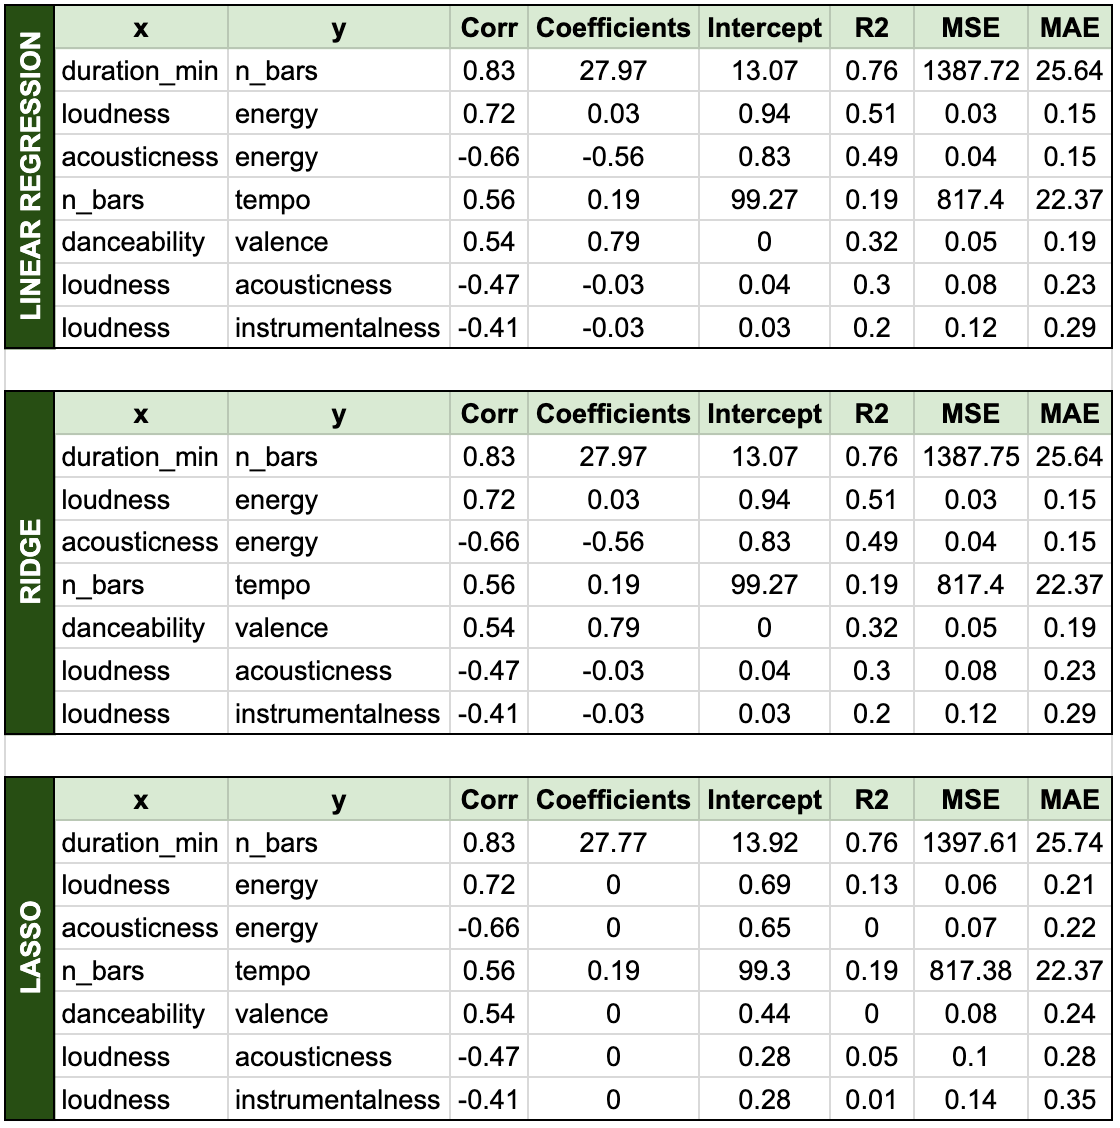
\includegraphics[width=.8\linewidth]{img/reg_1.png}
  \label{fig:test1}
  \centering
  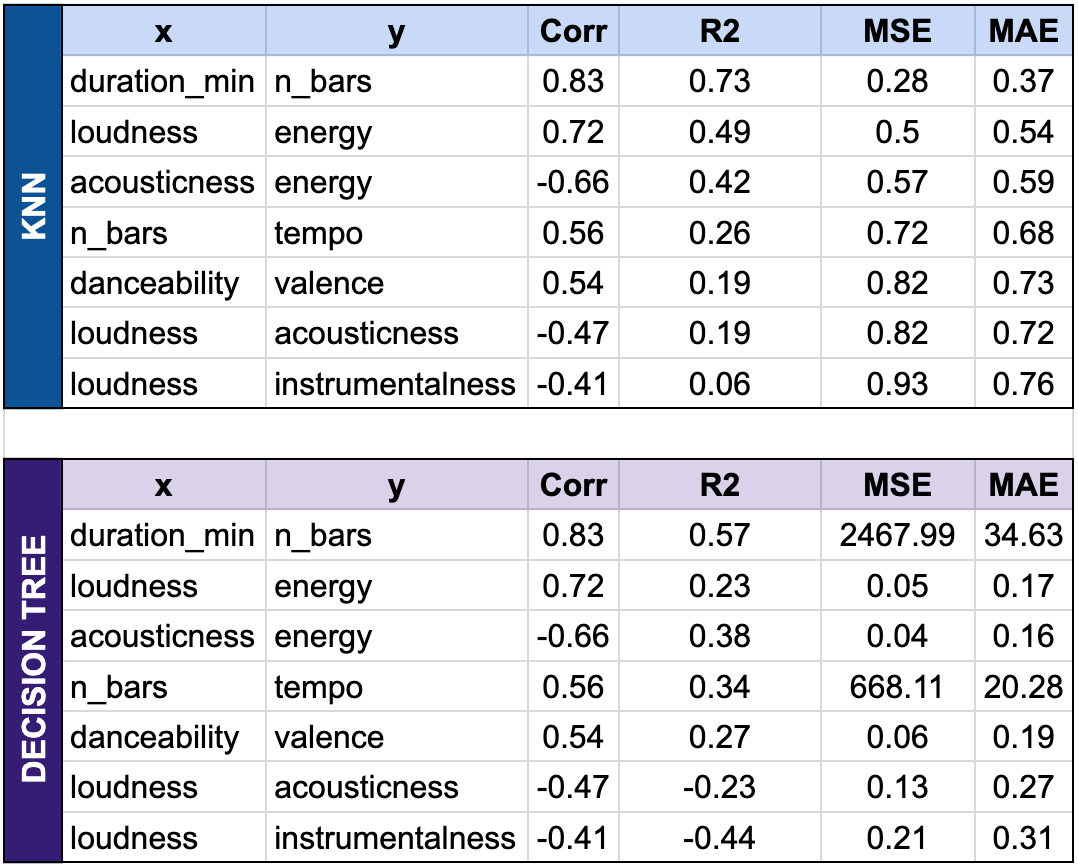
\includegraphics[width=.8\linewidth]{img/reg_2.png}
  \label{fig:test2}
\vspace{-1cm}
\end{wrapfigure}
\end{comment}

We created a function that performs simple linear regression using the provided regressor (that will be Linear, Ridge or Lasso) on the given training and testing datasets. It returns a dictionary containing the fitted model, its coefficients and intercept, and the $R^2$, $MSE$, and $MAE$ of the model on the test data. Then, for each regressor, our code performs a series of operations to identify pairs of features in a dataset that have a strong positive or negative correlation, and then applies simple linear regression to these pairs. After sorting the feature pairs based on the absolute value of their Spearman correlation coefficients, it filters the pairs to only include those with a correlation coefficient greater than $0.4$ or less than $-0.4$ (the threshold was chosen based on the values displayed in the correlation matrix). For each of these selected pairs, the code fits the model on the training data and uses it to predict the dependent variable in the test data. The list of results is converted into a pandas DataFrame that provides a comprehensive summary of the relationships between different features in the dataset and the performance of the model. In addition to the linear methods, we also used on the same pairs of features two previously seen models, KNN and DecisionTree, this time as regressors.
\begin{figure}[H]
\centering
\begin{minipage}{.5\textwidth}
  \centering
  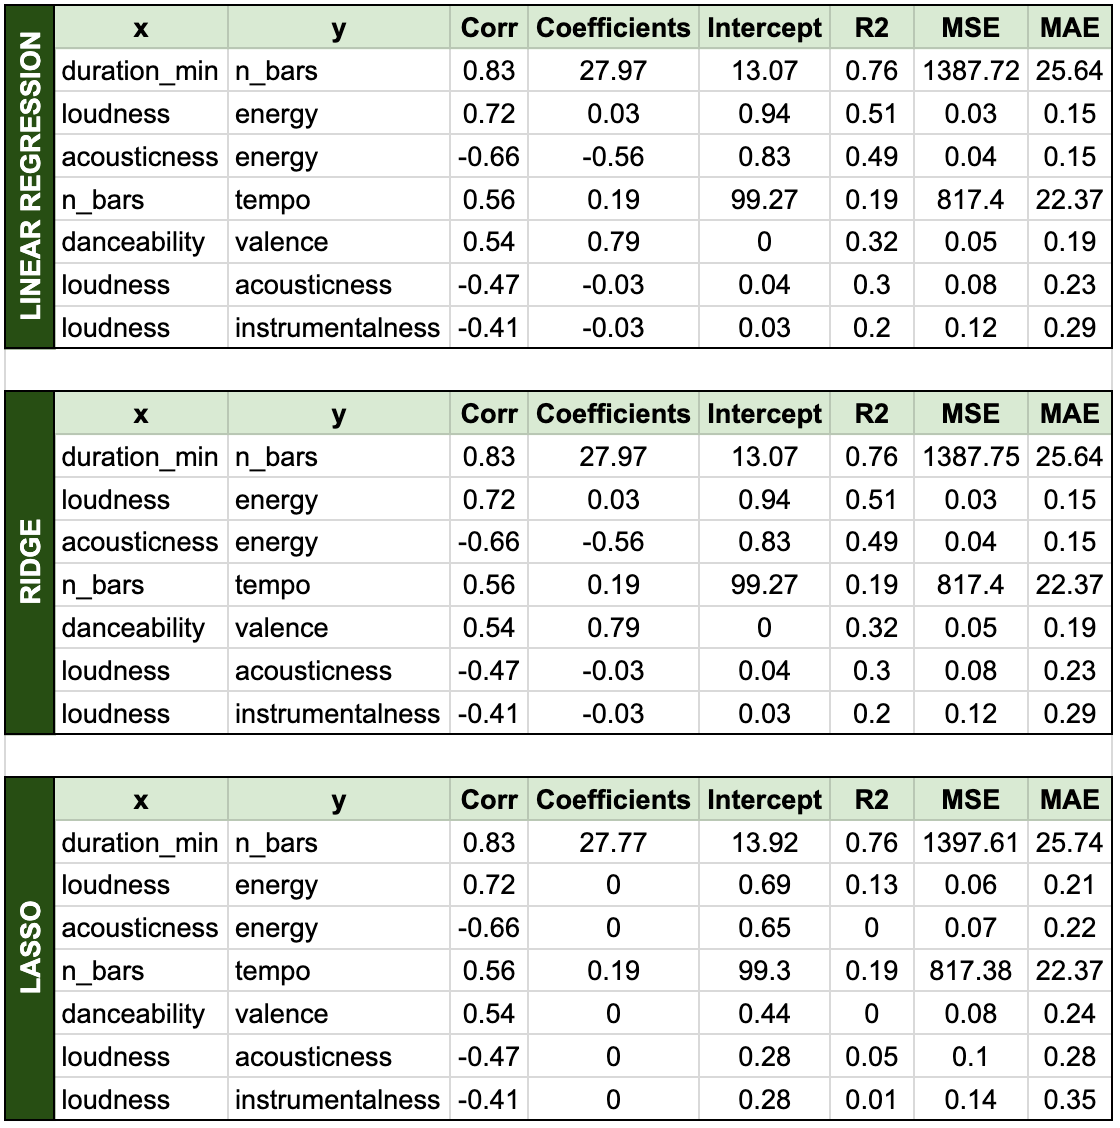
\includegraphics[width=.8\linewidth]{img/reg_1.png}
  \label{fig:test1}
\end{minipage}%
\begin{minipage}{.5\textwidth}
  \centering
  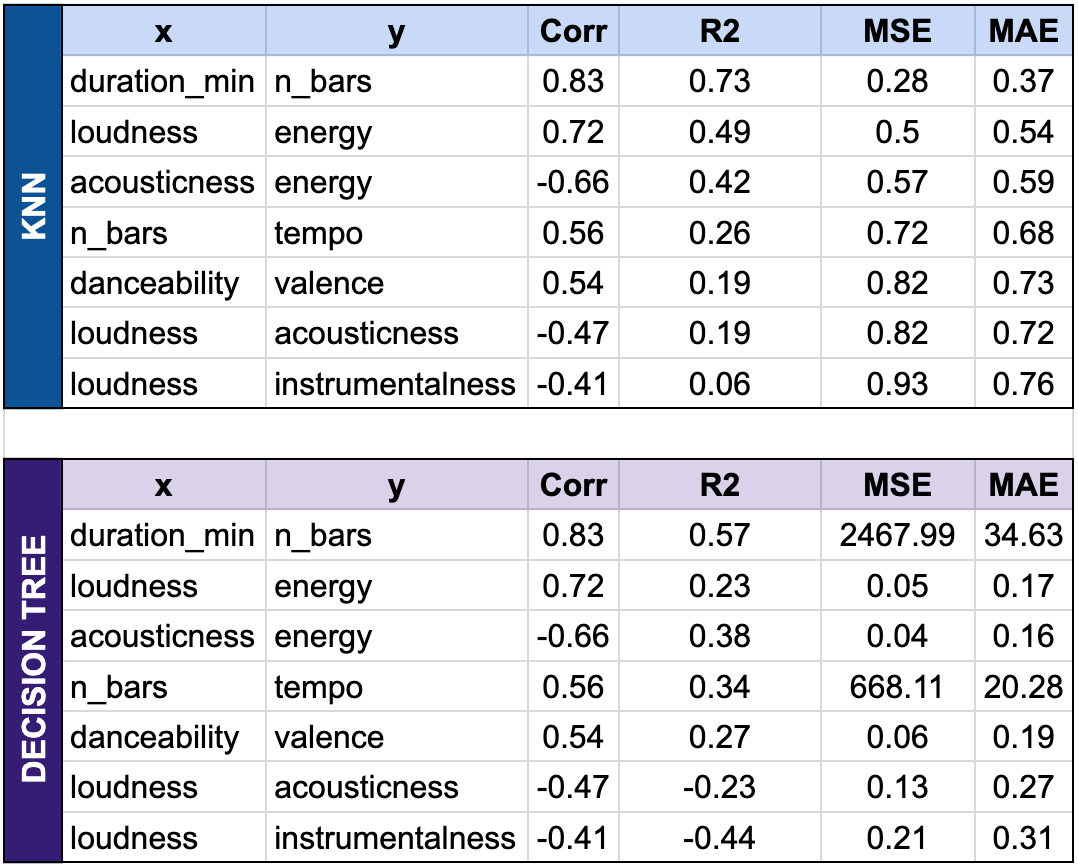
\includegraphics[width=.8\linewidth]{img/reg_2.png}
  \label{fig:test2}
\end{minipage}
\captionof{figure}{Results of linear and non-linear regression, performed on different pairs of features.}
\end{figure}
\noindent The best performing model is the one between duration\_min and n\_bars. This confirms what we expected, because the length of the song increases as the number of bars it contains increases. One of the worst performing models is the one between n\_bars and tempo. In fact, the number of bars in a song does not significantly influence its tempo, at least not in a linear way. The tempo and the number of beats of a song are largely independent musical elements: knowing the number of beats of a song does not provide much information about its tempo. The tempo of a piece is often chosen based on the mood or musical style, while the number of beats is typically determined by the structure and length of the piece.
\subsubsection{Multiple Regression}
We created a procedure that iterates over the list of targets containing only continuous variables of the dataset: the code, for each target, splits the dataset into train/test, standardizes the data, tests the different types of models seen above (performing a gridsearch based on the grid of parameters chosen) and then saves the results in a dataframe, sorting them by descending value of $R^2$.
\begin{figure}[H]
    \centering
    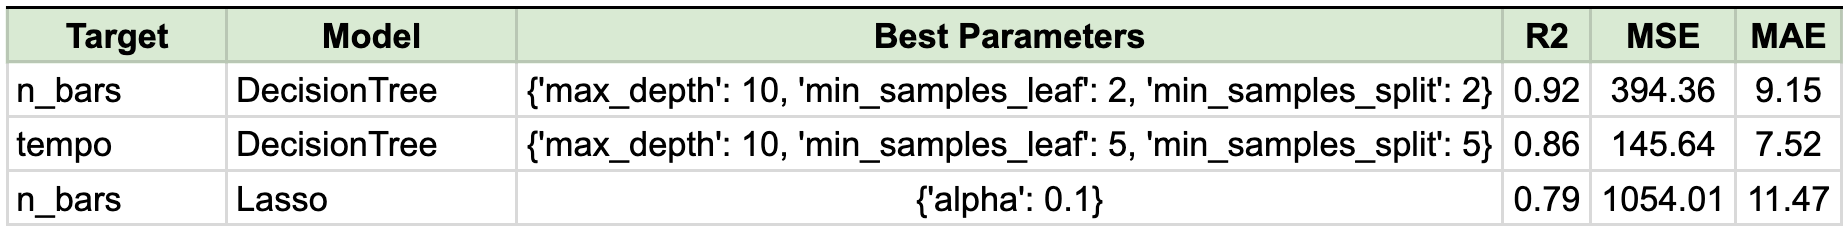
\includegraphics[scale=0.48]{img/multi_reg.png}
    \caption{Part of the results of multiple regression analysis: here we can see the 3 best combinations target-model.}
    \label{fig:enter-label}
\end{figure}
\subsubsection{Multivariate Regression}
As targets this time we have chosen: list \texttt{[popularity, danceability, energy]}, which can have implications in the music business, aiding in music recommendation, playlist creation, artist guidance, and advertising; then, after checking correlation to avoid multicollinearity, we added \texttt{[speechiness, acousticness, instrumentalness, liveness, valence]}, so that we can see performances with more targets.
\begin{figure}[H]
    \centering
    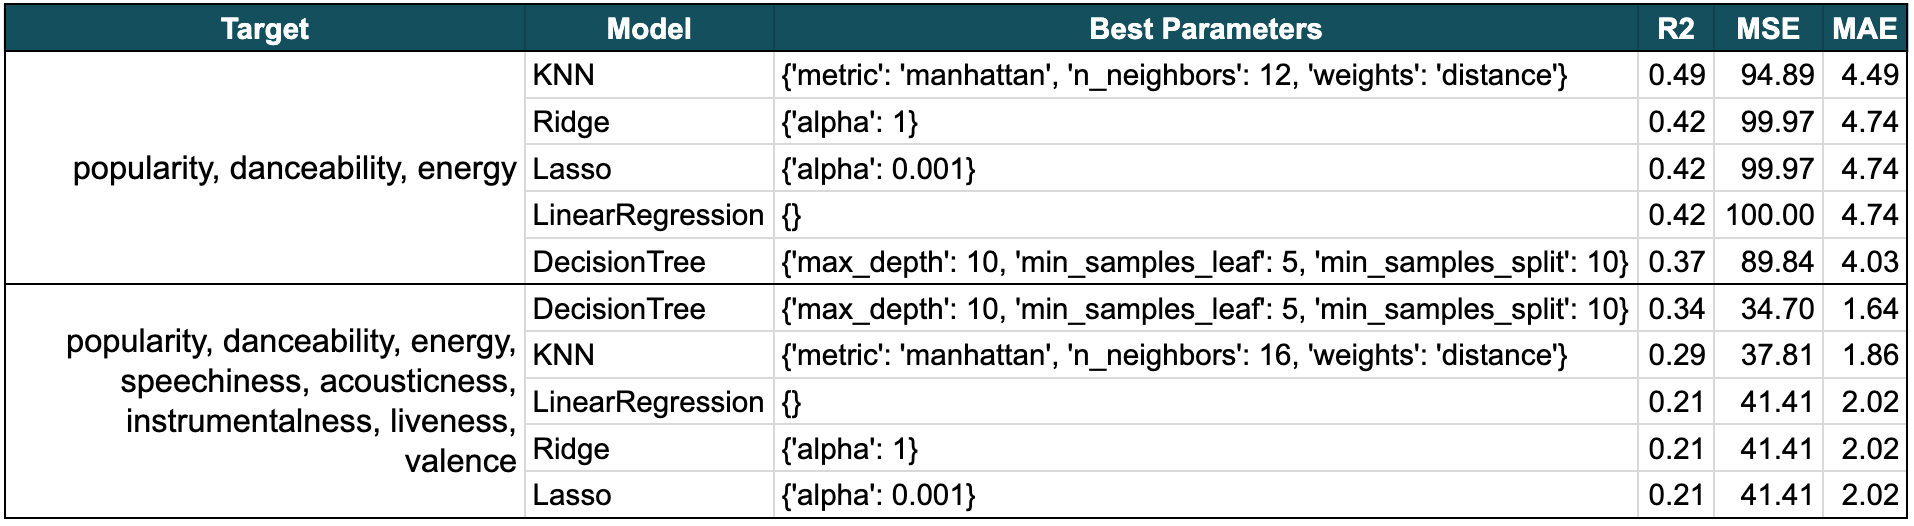
\includegraphics[scale=0.45]{img/multivariate.png}
    \caption{Results of the multivariate regression analysis.}
    \label{fig:enter-label}
\end{figure}
\section{Pattern Mining}
Before starting the analysis, we prepared the data: we mapped the categorical features to the actual values, for example, by substituting each key value for the corresponding Pitch Class Notation value (1 represents $C$ pitch, 2 represents $C\sharp/D\flat$, and so on); then we discretized the continuous variables, each in 3 bins, using \texttt{pd.cut}.
\subsection{Frequent Patterns}
\subsubsection*{Apriori}
Before running the Apriori algorithm, we looked for the optimal values of supp (minimum support of an item set) and zmin (minimum number of items per item set). The code defines a grid of parameters for the Apriori algorithm: \texttt{supp} values are generated using numpy’s linspace function to create 5 evenly spaced values between 10 and 50; \texttt{zmin} values are generated using numpy’s arange function to create a range of values from 5 to the number of columns in the dataframe. Then it runs the Apriori algorithm for each combination of \texttt{supp} and \texttt{zmin} values in the parameter grid, computing, for each combination, the number of frequent, closed, and maximal itemsets. Results are sorted by the number of frequent, closed, and maximal itemsets in descending order. The best configuration founded is \texttt{[supp=10, zmin=5]}. In fact, by setting 2, 3 or 4 as the minimum of the \texttt{zmin} range, we realized that the patterns found were just a simple confirmation of some information already found in data understanding: for example, in the dataset most of the tracks have a fairly short duration (the distribution is positively skewed). By setting a value of zmin equal to 5 instead, we can already begin to get more useful patterns.
\begin{figure}[H]
\centering
\begin{minipage}{.5\textwidth}
\centering
    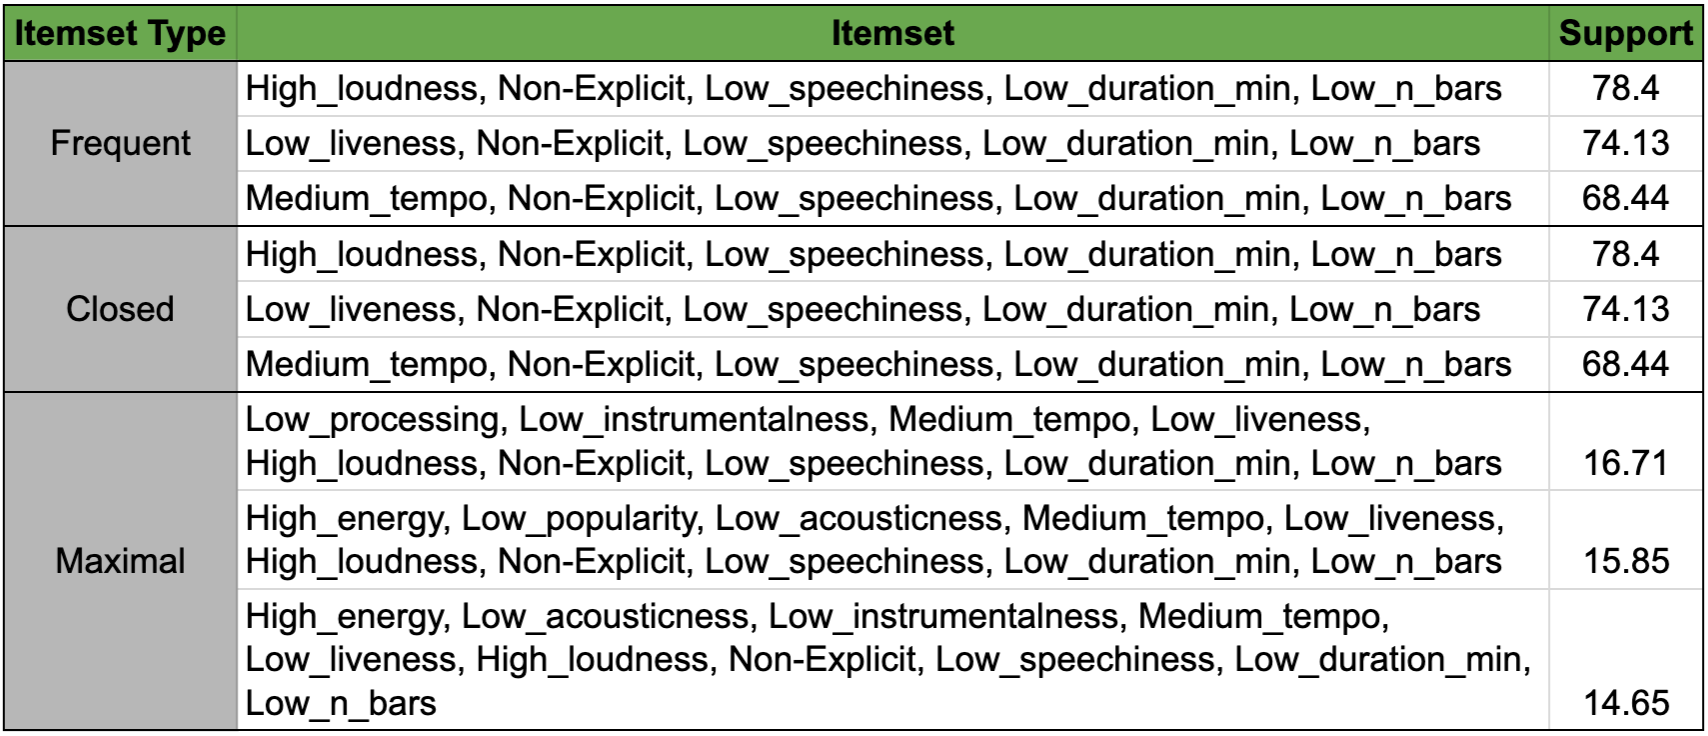
\includegraphics[width=\linewidth]{img/freqclosmax.png}
    \caption{Highest support values for the frequent, closed, and maximal itemsets derived from the Apriori algorithm.}
    \label{fig:enter-label}
\end{minipage}%
\hspace{0.5cm}
\begin{minipage}{.4\textwidth}
  \centering
  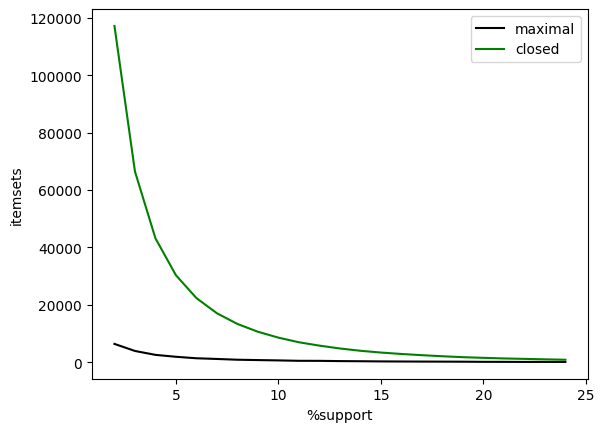
\includegraphics[width=.8\linewidth]{img/maxclos_plot.png}
  \caption{Number of maximal and closed itemsets (y-axis) for different support thresholds (x-axis).}
  \label{fig:test2}
\end{minipage}
\end{figure}
\noindent Our dataset predominantly consists of non-explicit tracks with high volume, low speechiness, a duration range that remains below 22 minutes, and a low number of bars. Tracks with medium tempo and low speechiness also have a significant presence. The presence of liveness feature among the most frequent patterns also suggests that dataset contains lots of tracks that have a low “live” feel.
\subsubsection*{FP-Growth}
We implemented the same procedure used for apriori, with the goal of finding the optimal values of supp and zmin, which are again \texttt{[supp=10, zmin=5]}. These are the three frequent patterns found with the highest support:\\
\begin{center}
\tiny{
\begin{tabular}[ht]
{|l|c|}
\hline
\textbf{Frequent Itemset} & \textbf{Support} \\
\hline
High\_loudness, Non-Explicit, Low\_speechiness, Low\_duration\_min, Low\_n\_bars & 78.4 \\
Low\_liveness, Non-Explicit, Low\_speechiness, Low\_duration\_min, Low\_n\_bars & 74.13 \\
Low\_liveness, High\_loudness, Low\_speechiness, Low\_duration\_min, Low\_n\_bars & 67.97 \\
\hline
\end{tabular}
}
\end{center}
\subsection{Association Rules}
We implemented a code that runs the Apriori algorithm for association rule mining over a range of confidence values (from 50 to 95) with a step of 5. For each \texttt{conf} value we then compute the average lift for the rules generated. We chose as optimal \texttt{conf} value the confidence level with the highest average lift. Finally, the code runs the Apriori algorithm again with the best confidence level and displays the resulting association rules sorted by lift in descending order.
\begin{figure}[H]
    \centering
    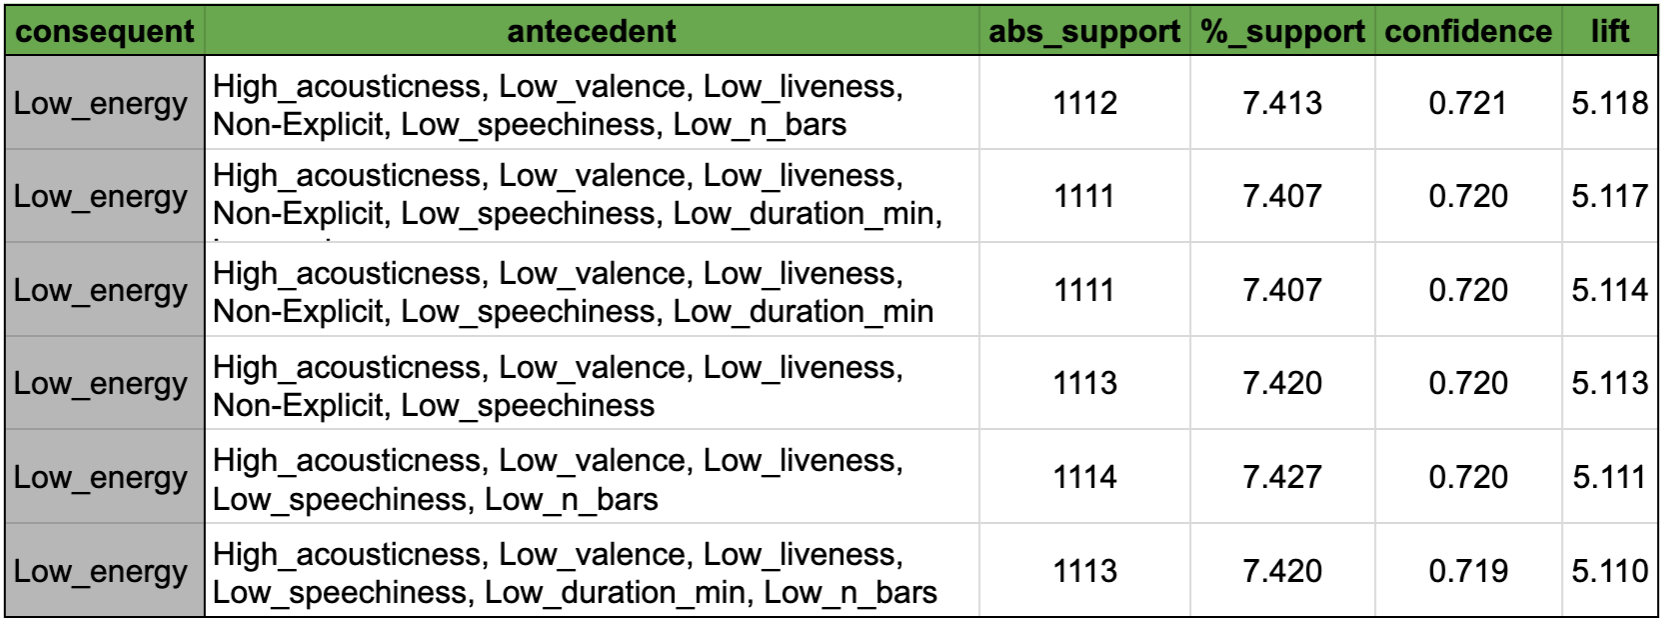
\includegraphics[scale=0.5]{img/rules.png}
    \caption{Association rules sorted by lift.}
    \label{fig:enter-label}
\end{figure}
We can see the following information:
\begin{itemize}
    \item Consequents: in our case it's mainly related to `energy`.
    \item Confidence: measures how often the rule has been found to be true. For example, a confidence of 0.72 for the first rule means that in about 72\% of the transactions containing [High\_acousticness, Low\_valence, Low\_liveness, Non-Explicit, Low\_speechiness, Low\_n\_bars] appear to have a low energy level.
    \item lift: ratio of the observed support to that expected if the antecedent and the consequent were independent. In our case, all the higher lifts are around 5, which means that the rules are quite significant.
\end{itemize}

The first rule can be read as: “If a relatively short song is acoustic, non-expicit and has low valence, liveness, speechiness, then it’s likely to have a low energy". This rule has a confidence of about 72\% and is about 5.1 times as likely to occur as would be expected if the conditions and result were independent. This pattern repeats for the other rules with slight variations in the conditions. All this also confirms the study of data understanding, in which we assumed such relationships based more or less only on correlations.

\end{document}